\chapter{Appendices}\label{chap:appendices}\label{chap:app-experiments}

%% ── Appendix A: Mathematical Notation ───────────────────────
\section{Mathematical Notation}\label{sec:appendix-a-mathematical-notation}

{\def\LTcaptype{table} % do not increment counter
\begin{longtable}[]{@{}ll@{}}
\toprule\noalign{}
Symbol & Description \\
\midrule\noalign{}
\endhead
\bottomrule\noalign{}
\endlastfoot
\(b\) & Binary bit (\(\in \{0, 1\}\)) \\
\(x\) & Modulated BPSK symbol (\(\in \{-1, +1\}\)) \\
\(y\) & Received signal \\
\(n\) & Noise sample \\
\(h\) & Fading coefficient \\
\(\sigma^2\) & Noise variance \\
\(\text{SNR}\) & Signal-to-Noise Ratio (linear) \\
\(G\) & AF amplification gain \\
\(\mathbf{H}\) & MIMO channel matrix (\(\in \mathbb{C}^{2 \times 2}\)) \\
\(\mathbf{W}\) & Neural network weight matrix \\
\(\mathbf{b}\) & Bias vector \\
\(P_e\) & Bit error rate \\
\(Q(\cdot)\) & Gaussian Q-function \\
\(K\) & Rician K-factor \\
\(\beta\) & VAE KL weight \\
\(\lambda\) & Regularization parameter \\
\(\eta\) & Learning rate \\
\(\Delta\) & State space discretization step \\
\(\mathbf{A}, \mathbf{B}, \mathbf{C}, D\) & State space model matrices \\
\end{longtable}
}

%% ── Appendix B: Model Architectures Summary Table ────────────
\section{Model Architectures and Hyperparameters}\label{sec:appendix-b-model-architectures-and-hyperparameters}

Table~\ref{tbl:arch-summary} summarises the key architectural parameters and training
settings for all nine relay strategies evaluated in this thesis.

\begin{table}[H]
\centering
\caption{Summary of relay architecture configurations and training hyperparameters.
All models trained with MSE loss (regression) or cross-entropy (16-class), Adam
optimiser, 100 epochs, 25\,000 training samples.}
\label{tbl:arch-summary}
\small
\begin{tabular}{@{}p{0.12\linewidth}p{0.08\linewidth}p{0.10\linewidth}p{0.28\linewidth}p{0.10\linewidth}p{0.12\linewidth}@{}}
\toprule
\textbf{Architecture} & \textbf{Params} & \textbf{Device} & \textbf{Key Structure} & \textbf{Output Act.} & \textbf{Train Time} \\
\midrule
AF & 0 & --- & Scale received signal by gain $G$ & --- & 0\,s \\
DF & 0 & --- & Hard-decision demodulate and re-modulate & --- & 0\,s \\
MLP (Minimal) & 169 & CPU & Window(5)$\to$24(ReLU)$\to$1 & tanh & 4.9\,s \\
Hybrid & 169 & CPU & MLP below SNR threshold; DF above & tanh & 4.6\,s \\
VAE & 1\,777 & CPU & Enc: 7$\to$32$\to$16$\to$\(\mu,\sigma^2\)(8); Dec: 8$\to$32$\to$1 & tanh & 21.6\,s \\
CGAN (WGAN-GP) & 2\,946 & CUDA & Gen: (7+8)$\to$32$\to$32$\to$16$\to$1; Critic: (1+7)$\to$32$\to$16$\to$1 & tanh & $\sim$2\,h \\
Transformer & 17\,697 & CUDA & 2 layers, 4 heads, $d_\text{model}$=32, $d_\text{ff}$=128 & tanh & $\sim$8\,min \\
Mamba S6 & 24\,001 & CUDA & 2 layers, expand 32$\to$64, $d_\text{state}$=16, selective $\Delta,B,C$ & tanh & $\sim$36\,min \\
Mamba-2 SSD & 26\,179 & CUDA & 2 layers, SSD kernel, chunk\_size=8, $d_\text{state}$=6 & tanh & $\sim$24\,min \\
\bottomrule
\end{tabular}
\end{table}

%% ── Appendix C: Software Architecture ───────────────────────
\section{Software Architecture}\label{sec:appendix-c-software-architecture}

The project is implemented as a modular Python package (\texttt{relaynet}) with the
architecture shown in Figure~\ref{fig:sw-architecture}. The design follows an
object-oriented pattern with a common \texttt{Relay} base class enabling polymorphic
relay swapping. Monte Carlo simulation is implemented in \texttt{runner.py} with
configurable trial count, bit count, and SNR range.

\begin{figure}[H]
\centering
\begin{tikzpicture}[
  pkg/.style={rectangle, draw=tauBlue, fill=tauBlue!10, rounded corners=4pt,
              minimum width=3.2cm, minimum height=0.7cm, font=\small\ttfamily,
              align=center},
  mod/.style={rectangle, draw=tauGray, fill=gray!8, rounded corners=2pt,
              minimum width=2.8cm, minimum height=0.55cm, font=\footnotesize\ttfamily,
              align=center},
  arr/.style={-Stealth, thick, tauBlue},
  grp/.style={rectangle, draw=tauGray!60, dashed, rounded corners=6pt,
              inner sep=6pt}
]

%% Top-level package
\node[pkg] (relaynet) at (0,0) {\textbf{relaynet}};

%% Sub-packages
\node[pkg] (channels)    at (-5.5,-1.8) {channels/};
\node[pkg] (modulation)  at (-1.8,-1.8) {modulation/};
\node[pkg] (relays)      at (1.8,-1.8)  {relays/};
\node[pkg] (simulation)  at (5.5,-1.8)  {simulation/};

%% Arrows from top to sub-packages
\draw[arr] (relaynet) -- (channels);
\draw[arr] (relaynet) -- (modulation);
\draw[arr] (relaynet) -- (relays);
\draw[arr] (relaynet) -- (simulation);

%% channels modules
\node[mod] (awgn)    at (-6.5,-3.2) {awgn.py};
\node[mod] (fading)  at (-5.5,-3.2) {fading.py};
\node[mod] (mimo)    at (-4.5,-3.2) {mimo.py};
\draw[arr] (channels) -- (awgn);
\draw[arr] (channels) -- (fading);
\draw[arr] (channels) -- (mimo);

%% modulation modules
\node[mod] (bpsk)  at (-2.6,-3.2) {bpsk.py};
\node[mod] (qpsk)  at (-1.8,-3.2) {qpsk.py};
\node[mod] (qam)   at (-1.0,-3.2) {qam.py};
\draw[arr] (modulation) -- (bpsk);
\draw[arr] (modulation) -- (qpsk);
\draw[arr] (modulation) -- (qam);

%% relays modules
\node[mod] (af)    at (0.6,-3.2)  {af.py};
\node[mod] (df)    at (1.4,-3.2)  {df.py};
\node[mod] (mlp)   at (2.2,-3.2)  {genai.py};
\node[mod] (vae)   at (3.0,-3.2)  {vae.py};
\draw[arr] (relays) -- (af);
\draw[arr] (relays) -- (df);
\draw[arr] (relays) -- (mlp);
\draw[arr] (relays) -- (vae);

%% simulation modules
\node[mod] (runner) at (5.0,-3.2) {runner.py};
\node[mod] (stats)  at (6.0,-3.2) {statistics.py};
\draw[arr] (simulation) -- (runner);
\draw[arr] (simulation) -- (stats);

%% Dependency arrows
\draw[arr, dashed, gray] (runner) to[bend right=20] node[below, font=\tiny] {uses} (relays);
\draw[arr, dashed, gray] (runner) to[bend right=30] node[below, font=\tiny] {uses} (channels);
\draw[arr, dashed, gray] (runner) to[bend right=40] node[below, font=\tiny] {uses} (modulation);

\end{tikzpicture}
\caption{Software architecture of the \texttt{relaynet} package. Solid arrows indicate
containment (sub-package or module); dashed arrows indicate runtime dependencies.
The \texttt{simulation/runner.py} orchestrates Monte Carlo BER evaluation by
composing channel, modulation, and relay components.}
\label{fig:sw-architecture}
\end{figure}

\textbf{Testing:} 126 automated tests (pytest) cover all channels, modulation schemes,
relay strategies, simulation, and statistics modules with 100\,\% pass rate.

\textbf{Reproducibility:} Random seeds are controlled at the bit-generation and
per-trial noise levels to ensure reproducible results.

%% ── Appendix D: Normalized 3K-Parameter Configurations ──────
\section{Normalised 3K-Parameter Configurations}\label{sec:appendix-d-normalized-3k-parameter-configurations}

{\def\LTcaptype{table} % do not increment counter
\begin{longtable}[]{@{}
  >{\raggedright\arraybackslash}p{(\linewidth - 6\tabcolsep) * \real{0.2500}}
  >{\raggedright\arraybackslash}p{(\linewidth - 6\tabcolsep) * \real{0.2500}}
  >{\raggedright\arraybackslash}p{(\linewidth - 6\tabcolsep) * \real{0.2500}}
  >{\raggedright\arraybackslash}p{(\linewidth - 6\tabcolsep) * \real{0.2500}}@{}}
\toprule\noalign{}
\begin{minipage}[b]{\linewidth}\raggedright
Model
\end{minipage} & \begin{minipage}[b]{\linewidth}\raggedright
Parameters
\end{minipage} & \begin{minipage}[b]{\linewidth}\raggedright
Window
\end{minipage} & \begin{minipage}[b]{\linewidth}\raggedright
Hidden / Architecture
\end{minipage} \\
\midrule\noalign{}
\endhead
\bottomrule\noalign{}
\endlastfoot
MLP-3K & 3,004 & 11 & hidden=231 \\
Hybrid-3K & 3,004 & 11 & hidden=231 (+ DF switch) \\
VAE-3K & 3,037 & 11 & latent=10, hidden=(44, 20) \\
CGAN-3K & 3,004 & 11 & noise=8, g\_hidden=(30, 30, 16), c\_hidden=(32, 16) \\
Transformer-3K & 3,007 & 11 & d\_model=18, heads=2, layers=1 \\
Mamba-3K & 3,027 & 11 & d\_model=16, d\_state=6, layers=1 \\
Mamba2-3K & 3,004 & 11 & d\_model=15, d\_state=6, chunk\_size=8, layers=1 \\
\end{longtable}
}

All 3K configurations use a window size of 11 to provide a common input context.
Parameter counts are within $\pm$1.2\,\% of the 3\,000-parameter target.


%% ── E1: Channel Model Validation ────────────────────────────
\section{E1: Channel Model Validation}\label{sec:app-e1}

\begin{figure}[H]
\centering
\pandocbounded{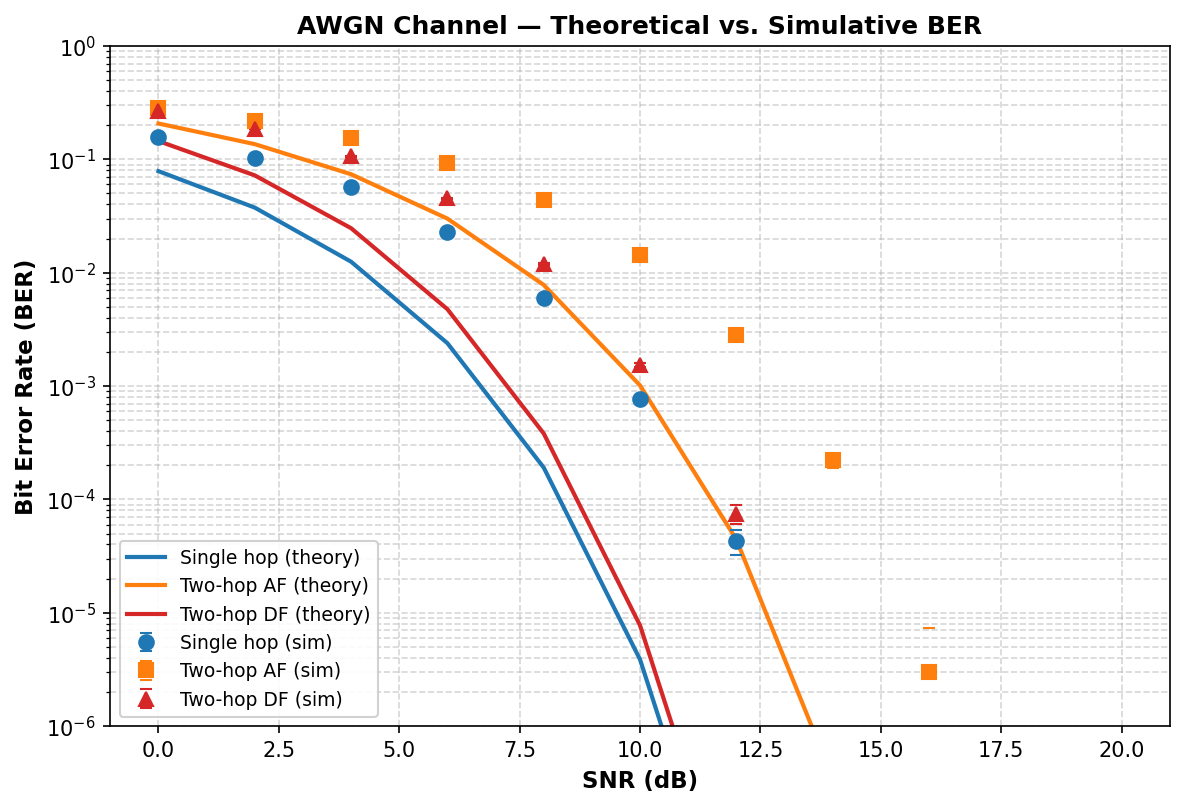
\includegraphics[width=\linewidth,height=0.45\textheight,keepaspectratio]{results/channel_theoretical_awgn.png}}
\caption{AWGN Channel --- Theoretical vs.\ Simulative BER. Theory (solid lines) and
Monte Carlo simulation (markers with 95\,\% CI) match within the confidence interval
at all SNR points.}
\label{fig:fig1}
\end{figure}

\begin{figure}[H]
\centering
\pandocbounded{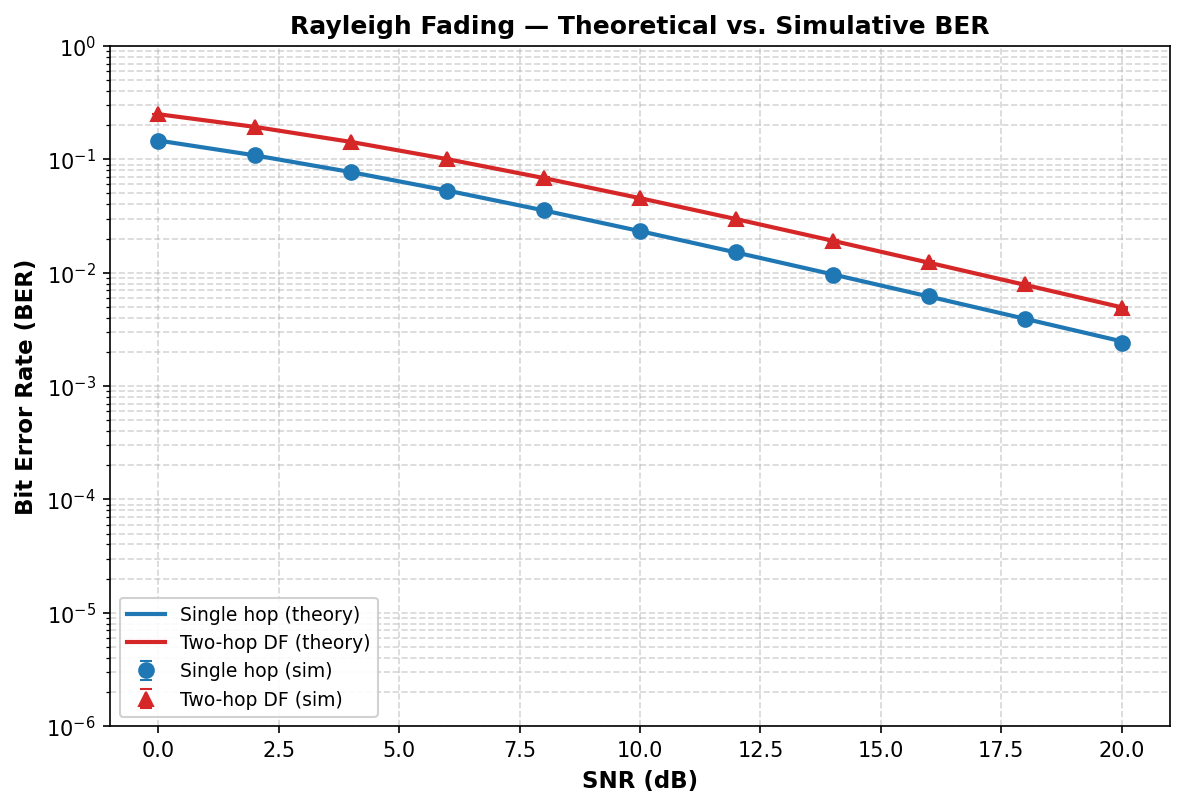
\includegraphics[width=\linewidth,height=0.45\textheight,keepaspectratio]{results/channel_theoretical_rayleigh.png}}
\caption{Rayleigh fading --- theory vs.\ simulation for single-hop and two-hop DF.
The characteristic $1/\text{SNR}$ slope is clearly visible.}
\label{fig:fig2}
\end{figure}

\begin{figure}[H]
\centering
\pandocbounded{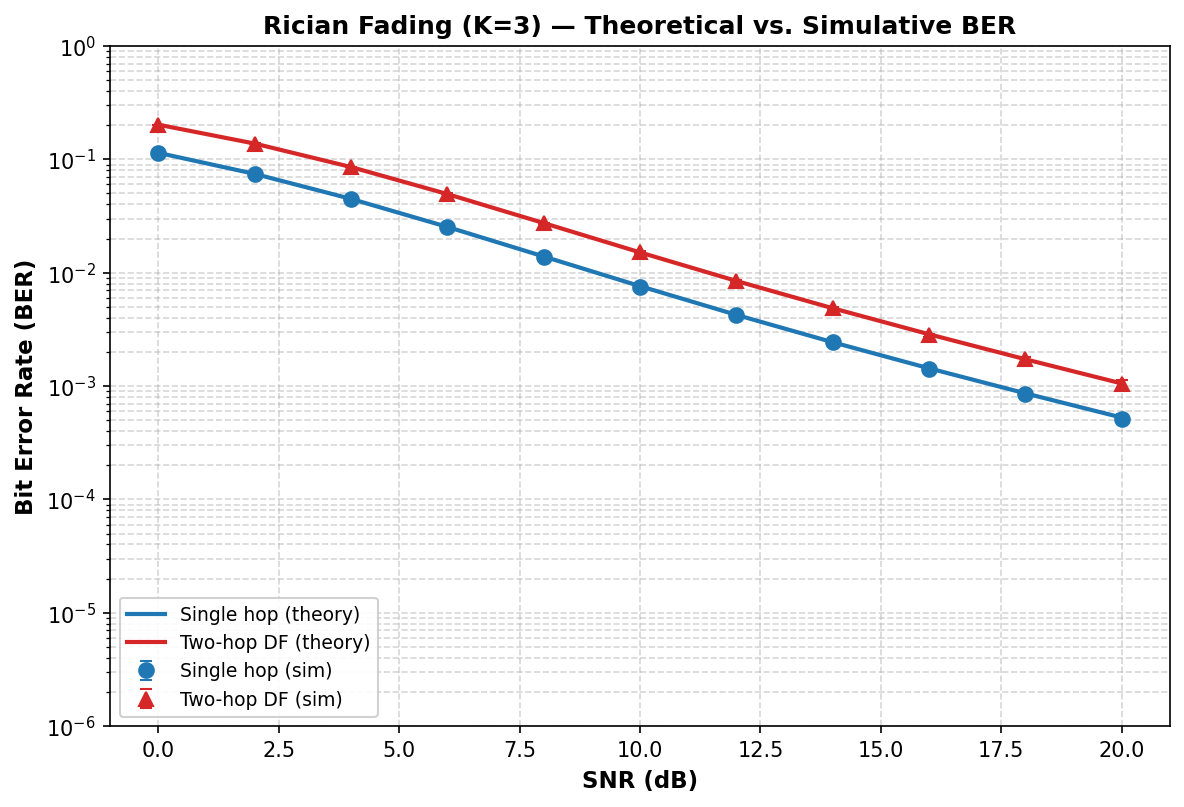
\includegraphics[width=\linewidth,height=0.45\textheight,keepaspectratio]{results/channel_theoretical_rician.png}}
\caption{Rician fading ($K{=}3$) --- theory vs.\ simulation for single-hop and two-hop DF.}
\label{fig:fig3}
\end{figure}

\begin{figure}[H]
\centering
\pandocbounded{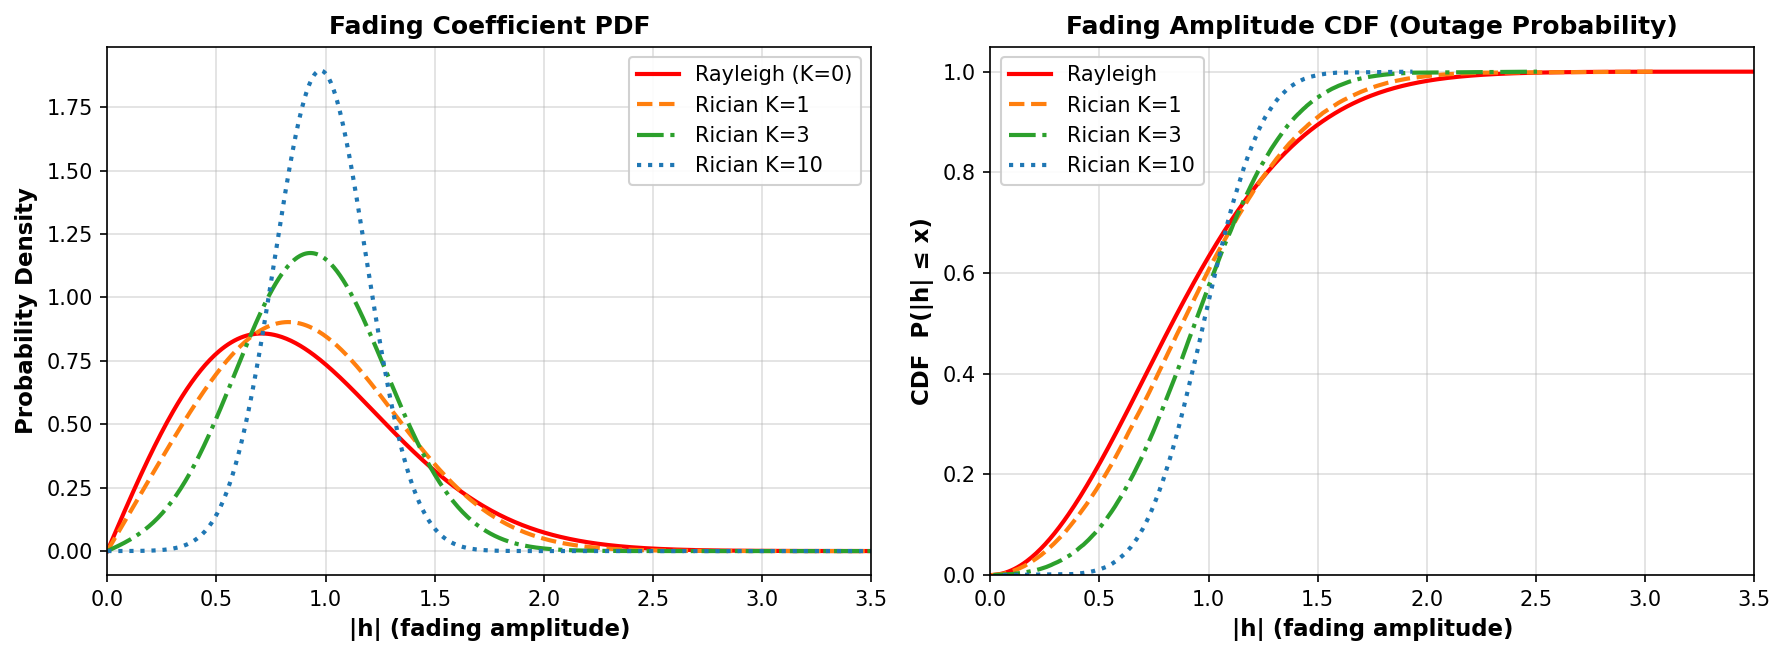
\includegraphics[width=\linewidth,height=0.45\textheight,keepaspectratio]{results/channel_fading_pdf.png}}
\caption{Left --- PDF of $|h|$ for Rayleigh and Rician ($K{=}1, 3, 10$). Right --- CDF
(outage probability). Rayleigh has the highest deep-fade probability at any threshold.}
\label{fig:fig4}
\end{figure}

\begin{figure}[H]
\centering
\pandocbounded{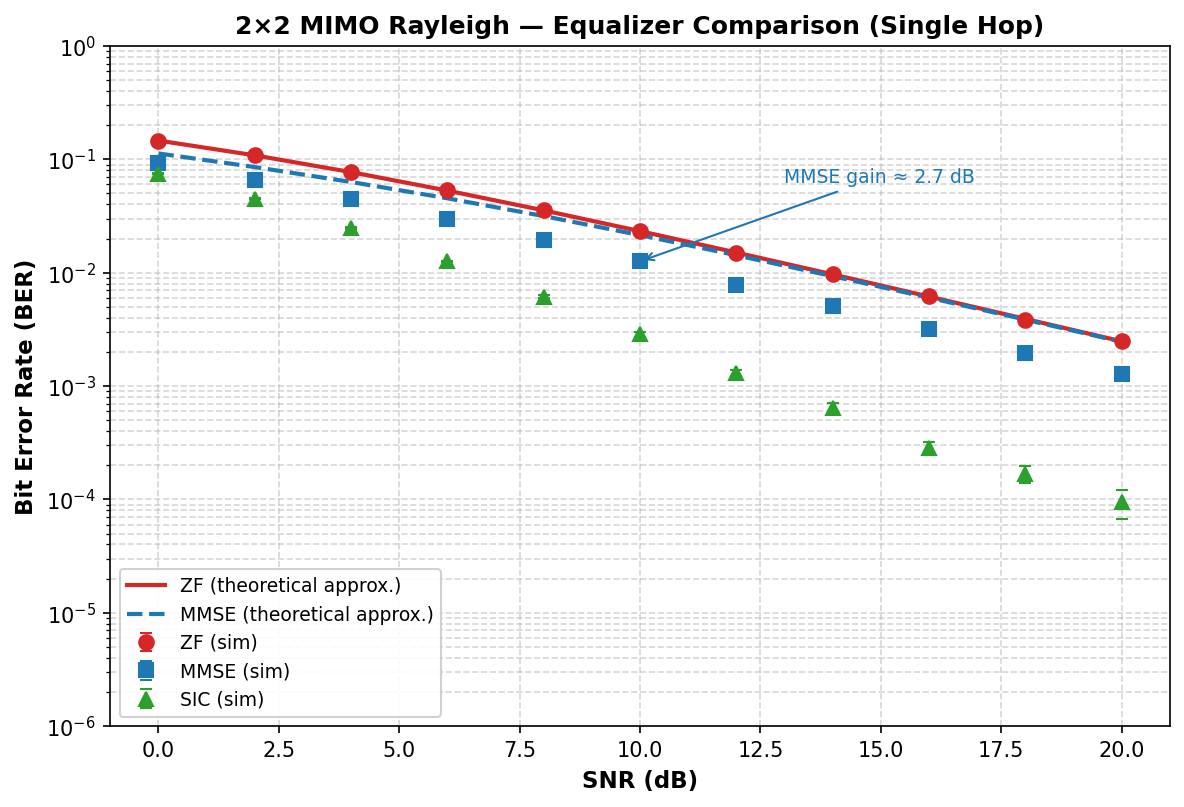
\includegraphics[width=\linewidth,height=0.45\textheight,keepaspectratio]{results/mimo_equalizer_comparison.png}}
\caption{2$\times$2 MIMO Rayleigh --- single-hop BER with ZF, MMSE, and SIC equalization.
MMSE provides $\sim$1--2\,dB gain over ZF; SIC provides an additional $\sim$0.5--1\,dB gain.}
\label{fig:fig5}
\end{figure}

\begin{figure}[H]
\centering
\pandocbounded{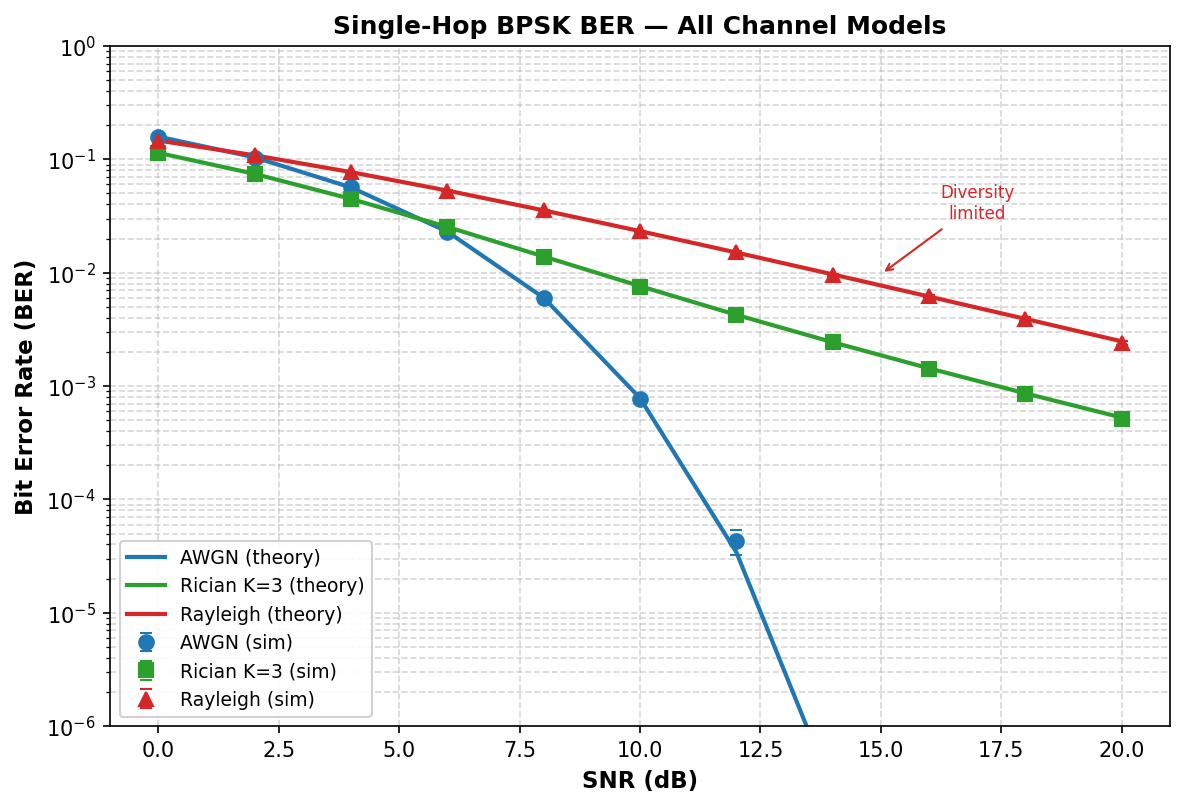
\includegraphics[width=\linewidth,height=0.45\textheight,keepaspectratio]{results/channel_comparison_all.png}}
\caption{Single-hop BPSK BER for all three SISO channel models. The SNR penalty for
Rayleigh relative to AWGN exceeds 15\,dB at BER $= 10^{-3}$.}
\label{fig:fig7}
\end{figure}


%% ── E2: SISO BPSK Baseline ───────────────────────────────────
\section{E2: SISO BPSK Performance (Baseline Relay Comparison)}\label{sec:app-e2}

\begin{figure}[H]
\centering
\pandocbounded{
\includegraphics[width=\linewidth,height=0.45\textheight,keepaspectratio]{results/awgn_comparison_ci.png}}
\caption{AWGN channel --- BER vs.\ SNR for all nine relay strategies with 95\,\% CI.
AI relays outperform classical methods at low SNR; DF dominates at medium-to-high SNR.}
\label{fig:fig9}
\end{figure}

\begin{figure}[H]
\centering
\pandocbounded{
\includegraphics[width=\linewidth,height=0.45\textheight,keepaspectratio]{results/fading_comparison.png}}
\caption{Rayleigh fading --- BER vs.\ SNR for all nine relay strategies with 95\,\% CI.}
\label{fig:fig10}
\end{figure}

\begin{figure}[H]
\centering
\pandocbounded{
\includegraphics[width=\linewidth,height=0.45\textheight,keepaspectratio]{results/rician_comparison_ci.png}}
\caption{Rician fading ($K{=}3$) --- BER vs.\ SNR for all nine relay strategies with 95\,\% CI.}
\label{fig:fig11}
\end{figure}


%% ── E3: MIMO 2x2 BPSK ───────────────────────────────────────
\section{E3: MIMO 2$\times$2 BPSK Performance}\label{sec:app-e3}

\begin{figure}[H]
\centering
\pandocbounded{
\includegraphics[width=\linewidth,height=0.45\textheight,keepaspectratio]{results/mimo_2x2_comparison_ci.png}}
\caption{2$\times$2 MIMO with ZF equalization --- BER vs.\ SNR for all nine relay strategies with 95\,\% CI.}
\label{fig:fig12}
\end{figure}

\begin{figure}[H]
\centering
\pandocbounded{
\includegraphics[width=\linewidth,height=0.45\textheight,keepaspectratio]{results/mimo_2x2_mmse_comparison_ci.png}}
\caption{2$\times$2 MIMO with MMSE equalization --- BER vs.\ SNR for all nine relay strategies with 95\,\% CI.}
\label{fig:fig13}
\end{figure}

\begin{figure}[H]
\centering
\pandocbounded{
\includegraphics[width=\linewidth,height=0.45\textheight,keepaspectratio]{results/mimo_2x2_sic_comparison_ci.png}}
\caption{2$\times$2 MIMO with MMSE-SIC equalization --- BER vs.\ SNR for all nine relay strategies with 95\,\% CI.}
\label{fig:fig14}
\end{figure}


%% ── E4: Parameter Normalisation ─────────────────────────────
\section{E4: Parameter Normalisation \& Complexity Trade-off}\label{sec:app-e4}

\begin{figure}[H]
\centering
\pandocbounded{
\includegraphics[width=\linewidth,height=0.45\textheight,keepaspectratio]{results/normalized_3k_all_channels.png}}
\caption{Normalised 3K-parameter comparison across all channels. At equal parameter
budgets, all architectures converge to similar BER, with VAE being the consistent
underperformer.}
\label{fig:fig15}
\end{figure}

\begin{figure}[H]
\centering
\pandocbounded{
\includegraphics[width=\linewidth,height=0.45\textheight,keepaspectratio]{results/normalized_3k_awgn.png}}
\caption{Normalised 3K-parameter BER comparison on AWGN. Mamba-3K and Transformer-3K
produce nearly identical BER, eliminating the gap seen at original parameter counts.}
\label{fig:fig16}
\end{figure}

\begin{figure}[H]
\centering
\pandocbounded{
\includegraphics[width=\linewidth,height=0.45\textheight,keepaspectratio]{results/normalized_3k_rayleigh.png}}
\caption{Normalised 3K-parameter BER comparison on Rayleigh fading.}
\label{fig:fig17}
\end{figure}

\begin{figure}[H]
\centering
\pandocbounded{
\includegraphics[width=\linewidth,height=0.45\textheight,keepaspectratio]{results/normalized_3k_rician_k3.png}}
\caption{Normalised 3K-parameter BER comparison on Rician fading ($K{=}3$).}
\label{fig:fig18}
\end{figure}

\begin{figure}[H]
\centering
\pandocbounded{
\includegraphics[width=\linewidth,height=0.45\textheight,keepaspectratio]{results/complexity_comparison_all_relays.png}}
\caption{Complexity--performance trade-off. Training time vs.\ parameter count vs.\
BER improvement over DF at low SNR. The Minimal MLP (169 params) achieves the best
efficiency.}
\label{fig:fig19}
\end{figure}

\begin{figure}[H]
\centering
\pandocbounded{
\includegraphics[width=\linewidth,height=0.45\textheight,keepaspectratio]{results/master_ber_comparison.png}}
\caption{Master BER comparison --- consolidated view of all nine relay strategies
across all six channel/topology configurations.}
\label{fig:fig20}
\end{figure}


%% ── E5: Higher-Order Modulation ─────────────────────────────
\section{E5: Higher-Order Modulation Scalability (Constellation-Aware Training)}\label{sec:app-e5}

\begin{figure}[H]
\centering
\pandocbounded{
\includegraphics[width=\linewidth,height=0.45\textheight,keepaspectratio]{results/modulation/bpsk_awgn_ci.png}}
\caption{BPSK on AWGN --- all relay strategies with 95\,\% CI (baseline for modulation comparison).}
\label{fig:fig21}
\end{figure}

\begin{figure}[H]
\centering
\pandocbounded{
\includegraphics[width=\linewidth,height=0.45\textheight,keepaspectratio]{results/modulation/bpsk_rayleigh_ci.png}}
\caption{BPSK on Rayleigh fading --- all relay strategies with 95\,\% CI.}
\label{fig:fig22}
\end{figure}

\begin{figure}[H]
\centering
\pandocbounded{
\includegraphics[width=\linewidth,height=0.45\textheight,keepaspectratio]{results/modulation/qpsk_awgn_ci.png}}
\caption{QPSK on AWGN --- BER curves closely match the BPSK baseline, confirming I/Q splitting validity.}
\label{fig:fig23}
\end{figure}

\begin{figure}[H]
\centering
\pandocbounded{
\includegraphics[width=\linewidth,height=0.45\textheight,keepaspectratio]{results/modulation/qpsk_rayleigh_ci.png}}
\caption{QPSK on Rayleigh fading --- same relative ordering as BPSK.}
\label{fig:fig24}
\end{figure}

\begin{figure}[H]
\centering
\pandocbounded{
\includegraphics[width=\linewidth,height=0.45\textheight,keepaspectratio]{results/modulation/qam16__awgn_ci.png}}
\caption{16-QAM on AWGN --- AI relays hit a BER floor near 0.22 at medium-high SNR
due to \texttt{tanh} compression of multi-level signals.}
\label{fig:fig25}
\end{figure}

\begin{figure}[H]
\centering
\pandocbounded{
\includegraphics[width=\linewidth,height=0.45\textheight,keepaspectratio]{results/modulation/qam16__rayleigh_ci.png}}
\caption{16-QAM on Rayleigh fading --- wider BER gap; all AI relays significantly
worse than DF at every SNR point.}
\label{fig:fig26}
\end{figure}

\begin{figure}[H]
\centering
\pandocbounded{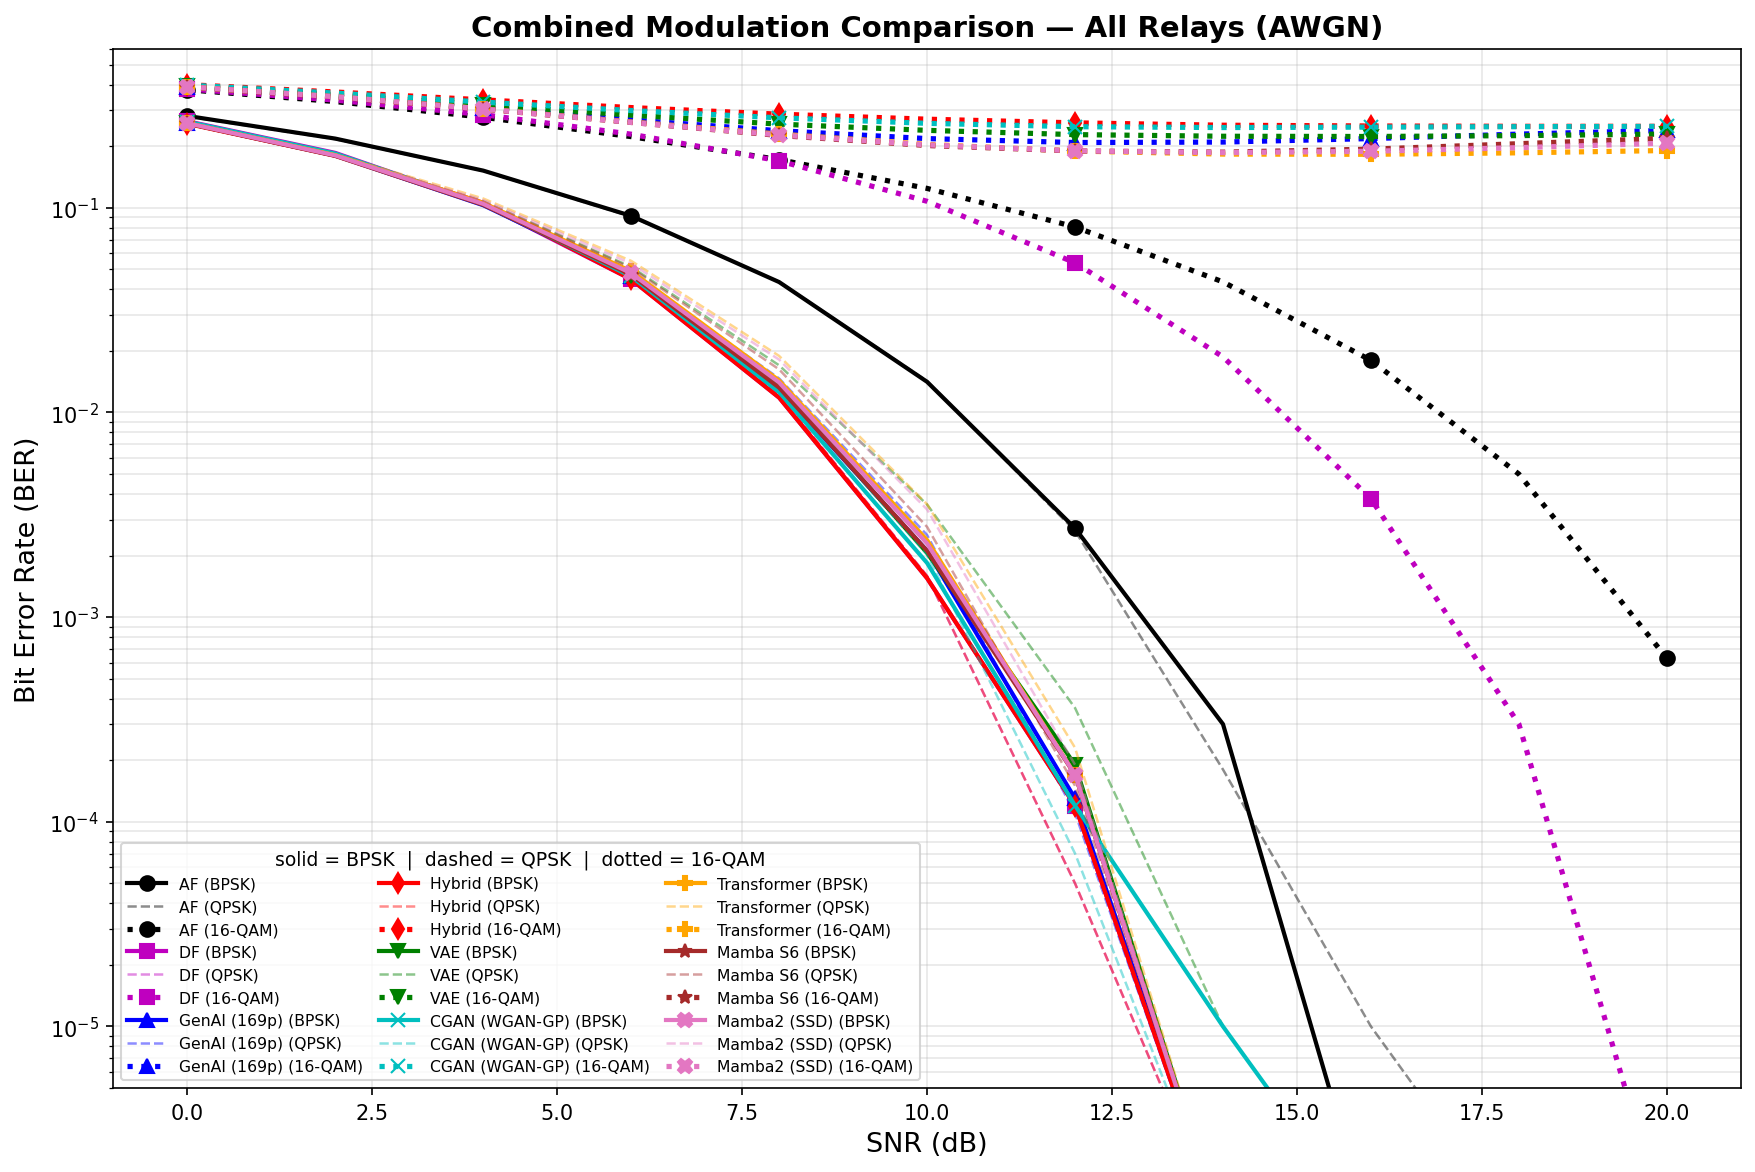
\includegraphics[width=\linewidth,height=0.45\textheight,keepaspectratio]{results/modulation/combined_modulation_awgn.png}}
\caption{Combined modulation comparison (AWGN) --- all nine relays across BPSK (solid),
QPSK (dashed), and 16-QAM (dotted). The BPSK/QPSK overlap confirms I/Q splitting
equivalence.}
\label{fig:fig27}
\end{figure}

\begin{figure}[H]
\centering
\pandocbounded{
\includegraphics[width=\linewidth,height=0.45\textheight,keepaspectratio]{results/qam16_activation/qam16_activation_awgn.png}}
\caption{16-QAM activation experiment (AWGN) --- replacing \texttt{tanh} and retraining
on QAM16 eliminates the BER floor for all AI relays except Hybrid.}
\label{fig:fig28}
\end{figure}

\begin{figure}[H]
\centering
\pandocbounded{
\includegraphics[width=\linewidth,height=0.45\textheight,keepaspectratio]{results/qam16_activation/qam16_activation_rayleigh.png}}
\caption{16-QAM activation experiment (Rayleigh fading) --- same trend under fading.}
\label{fig:fig29}
\end{figure}

\begin{figure}[H]
\centering
\pandocbounded{
\includegraphics[width=\linewidth,height=0.45\textheight,keepaspectratio]{results/activation_comparison/bpsk_activation_awgn.png}}
\caption{BPSK constellation-aware activation comparison (AWGN). All three bounded
activations achieve equivalent BER, confirming BPSK is insensitive to activation choice.}
\label{fig:fig30}
\end{figure}

\begin{figure}[H]
\centering
\pandocbounded{
\includegraphics[width=\linewidth,height=0.45\textheight,keepaspectratio]{results/activation_comparison/bpsk_activation_rayleigh.png}}
\caption{BPSK constellation-aware activation comparison (Rayleigh fading).}
\label{fig:fig31}
\end{figure}

\begin{figure}[H]
\centering
\pandocbounded{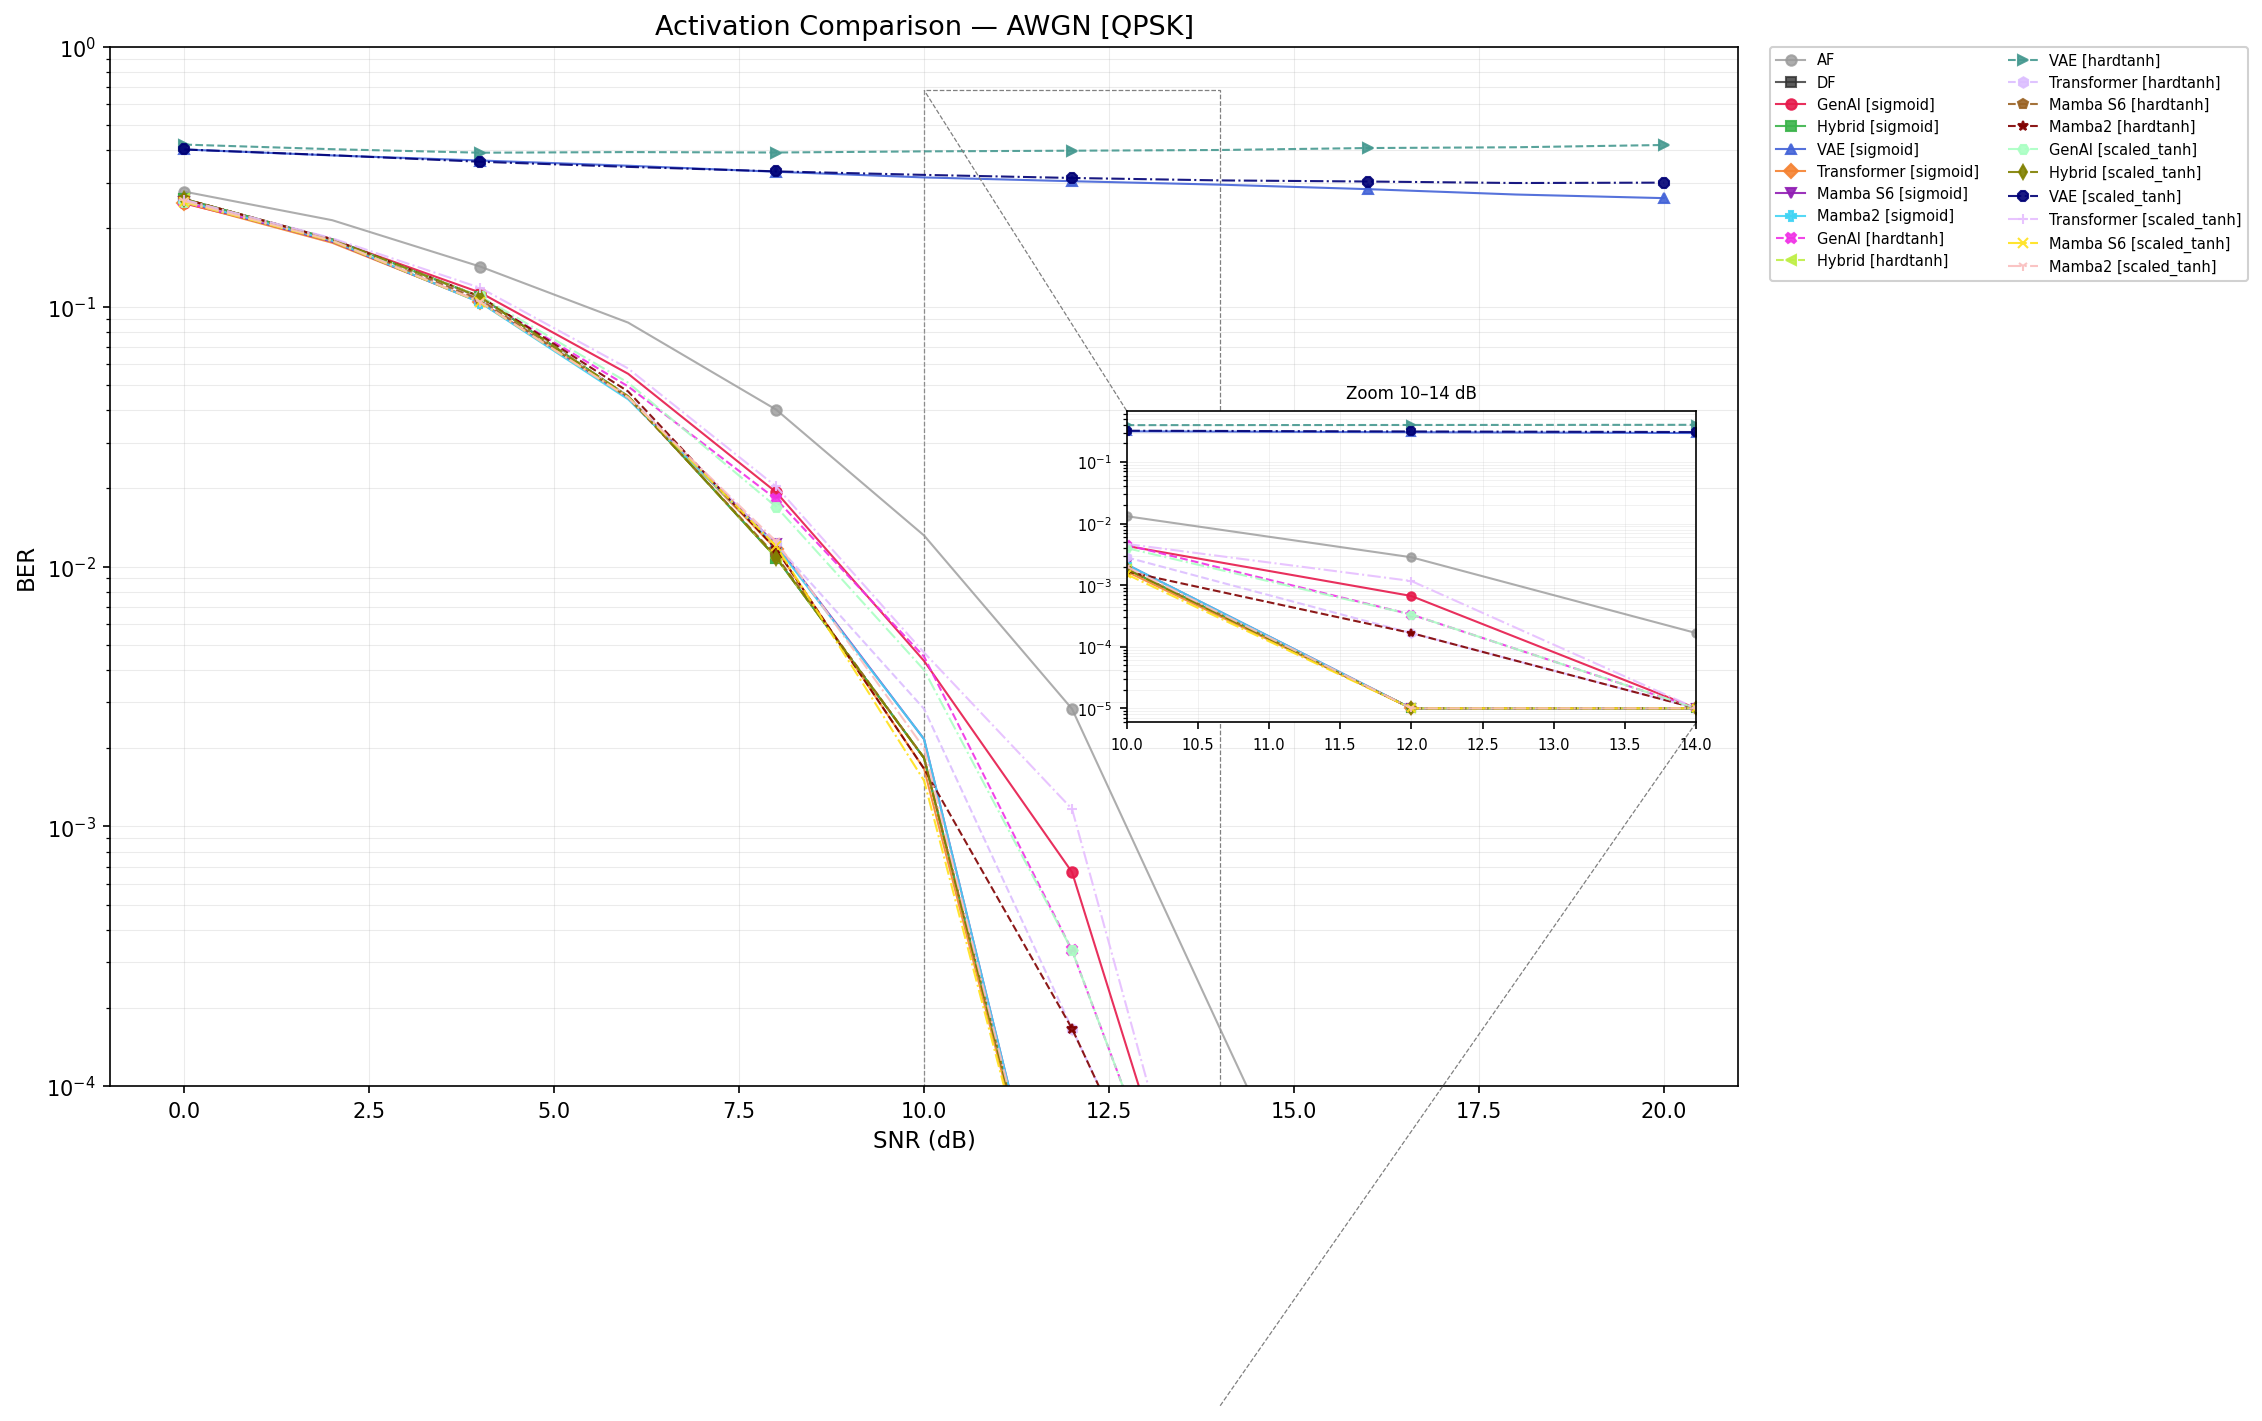
\includegraphics[width=\linewidth,height=0.45\textheight,keepaspectratio]{results/activation_comparison/qpsk_activation_awgn.png}}
\caption{QPSK constellation-aware activation comparison (AWGN).}
\label{fig:fig32}
\end{figure}

\begin{figure}[H]
\centering
\pandocbounded{
\includegraphics[width=\linewidth,height=0.45\textheight,keepaspectratio]{results/activation_comparison/qpsk_activation_rayleigh.png}}
\caption{QPSK constellation-aware activation comparison (Rayleigh fading).}
\label{fig:fig33}
\end{figure}

\begin{figure}[H]
\centering
\pandocbounded{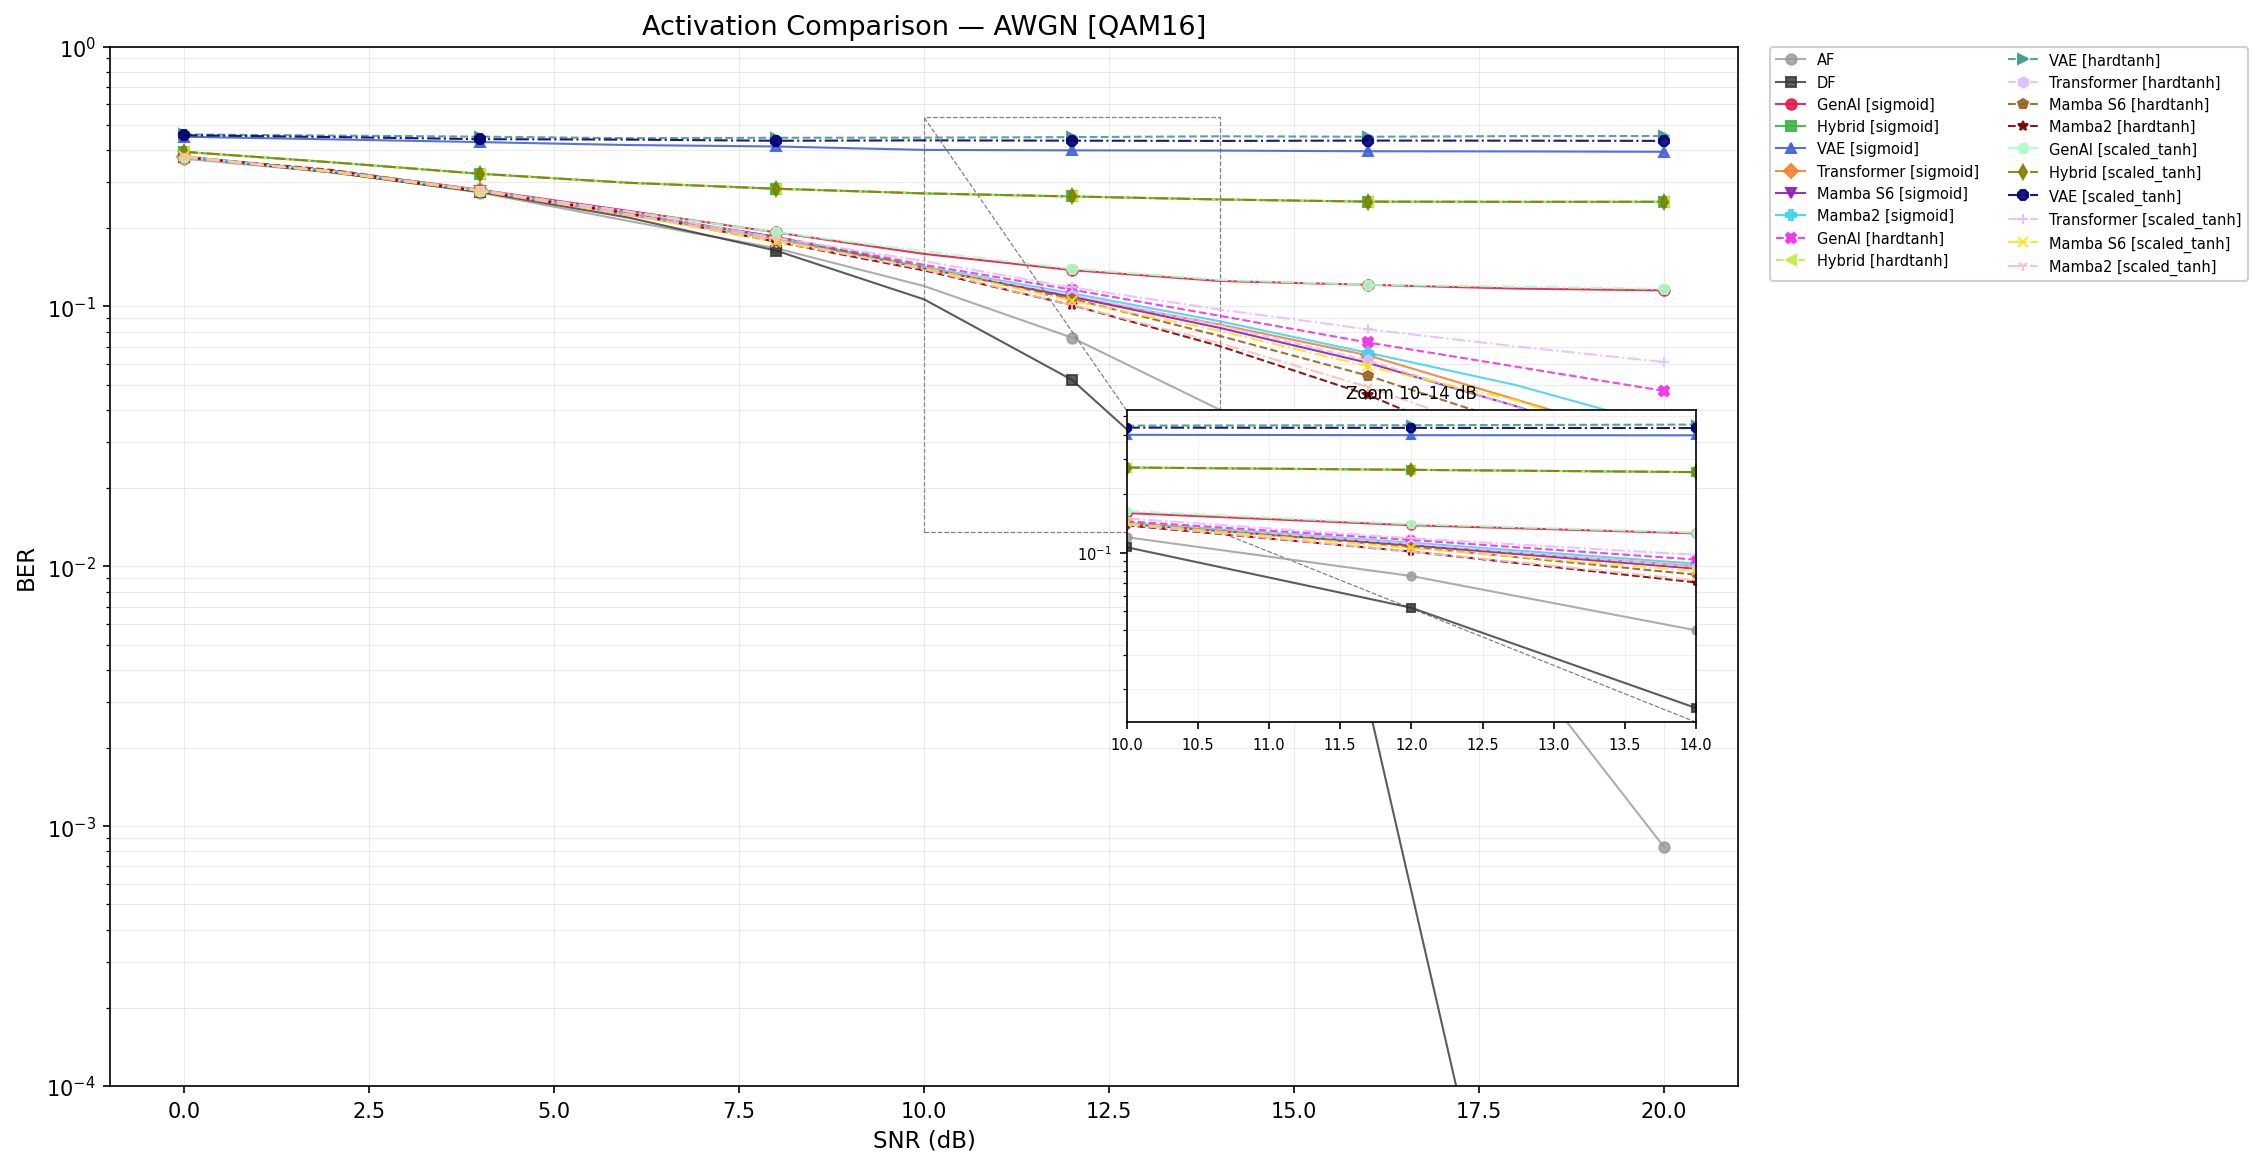
\includegraphics[width=\linewidth,height=0.45\textheight,keepaspectratio]{results/activation_comparison/qam16_activation_awgn.png}}
\caption{16-QAM constellation-aware activation comparison (AWGN). All three bounded
activations eliminate the \texttt{tanh} BER floor.}
\label{fig:fig34}
\end{figure}

\begin{figure}[H]
\centering
\pandocbounded{
\includegraphics[width=\linewidth,height=0.45\textheight,keepaspectratio]{results/activation_comparison/qam16_activation_rayleigh.png}}
\caption{16-QAM constellation-aware activation comparison (Rayleigh fading).}
\label{fig:fig35}
\end{figure}

\begin{figure}[H]
\centering
\pandocbounded{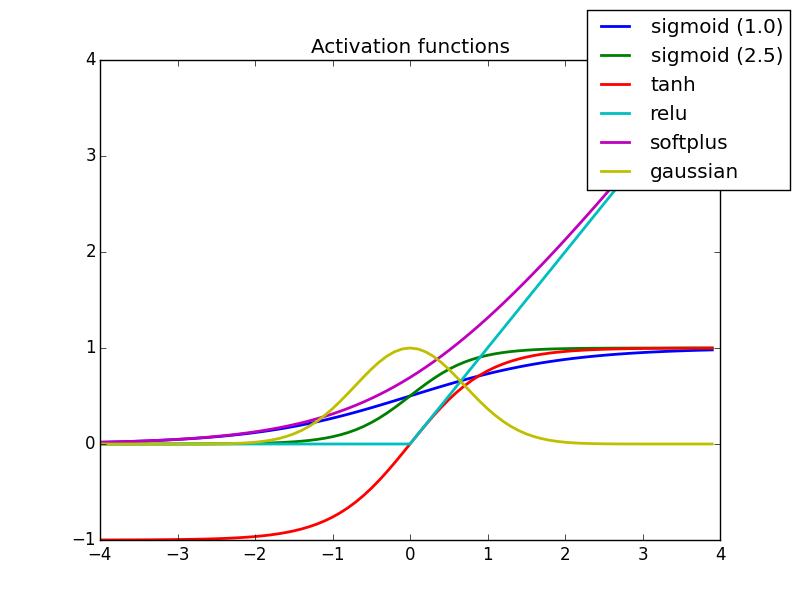
\includegraphics[width=\linewidth,height=0.45\textheight,keepaspectratio]{results/activation_comparison/various_activation_functions.png}}
\caption{Comparison of activation function shapes (left) and their derivatives (right)
for $A_{\max} = 0.9487$ (16-QAM).}
\label{fig:fig36}
\end{figure}


%% ── E6: CSI Injection & LayerNorm ───────────────────────────
\section{E6: Input Normalisation and CSI Injection}\label{chap:app-csi}

\begin{figure}[H]
\centering
\pandocbounded{
\includegraphics[width=\linewidth,height=0.45\textheight,keepaspectratio]{results/csi/csi_experiment_qam16_rayleigh.png}}
\caption{16-QAM Rayleigh fading --- BER vs.\ SNR for all 48 neural relay variants and
two classical baselines (AF, DF) with 95\,\% confidence intervals.}
\label{fig:fig39}
\end{figure}

\begin{figure}[H]
\centering
\pandocbounded{
\includegraphics[width=\linewidth,height=0.45\textheight,keepaspectratio]{results/csi/top3_qam16_rayleigh.png}}
\caption{Top-3 neural relay architectures for 16-QAM in Rayleigh fading. All three
best-performing variants use input LayerNorm (+LN) without CSI injection.}
\label{fig:fig40}
\end{figure}

\begin{figure}[H]
\centering
\pandocbounded{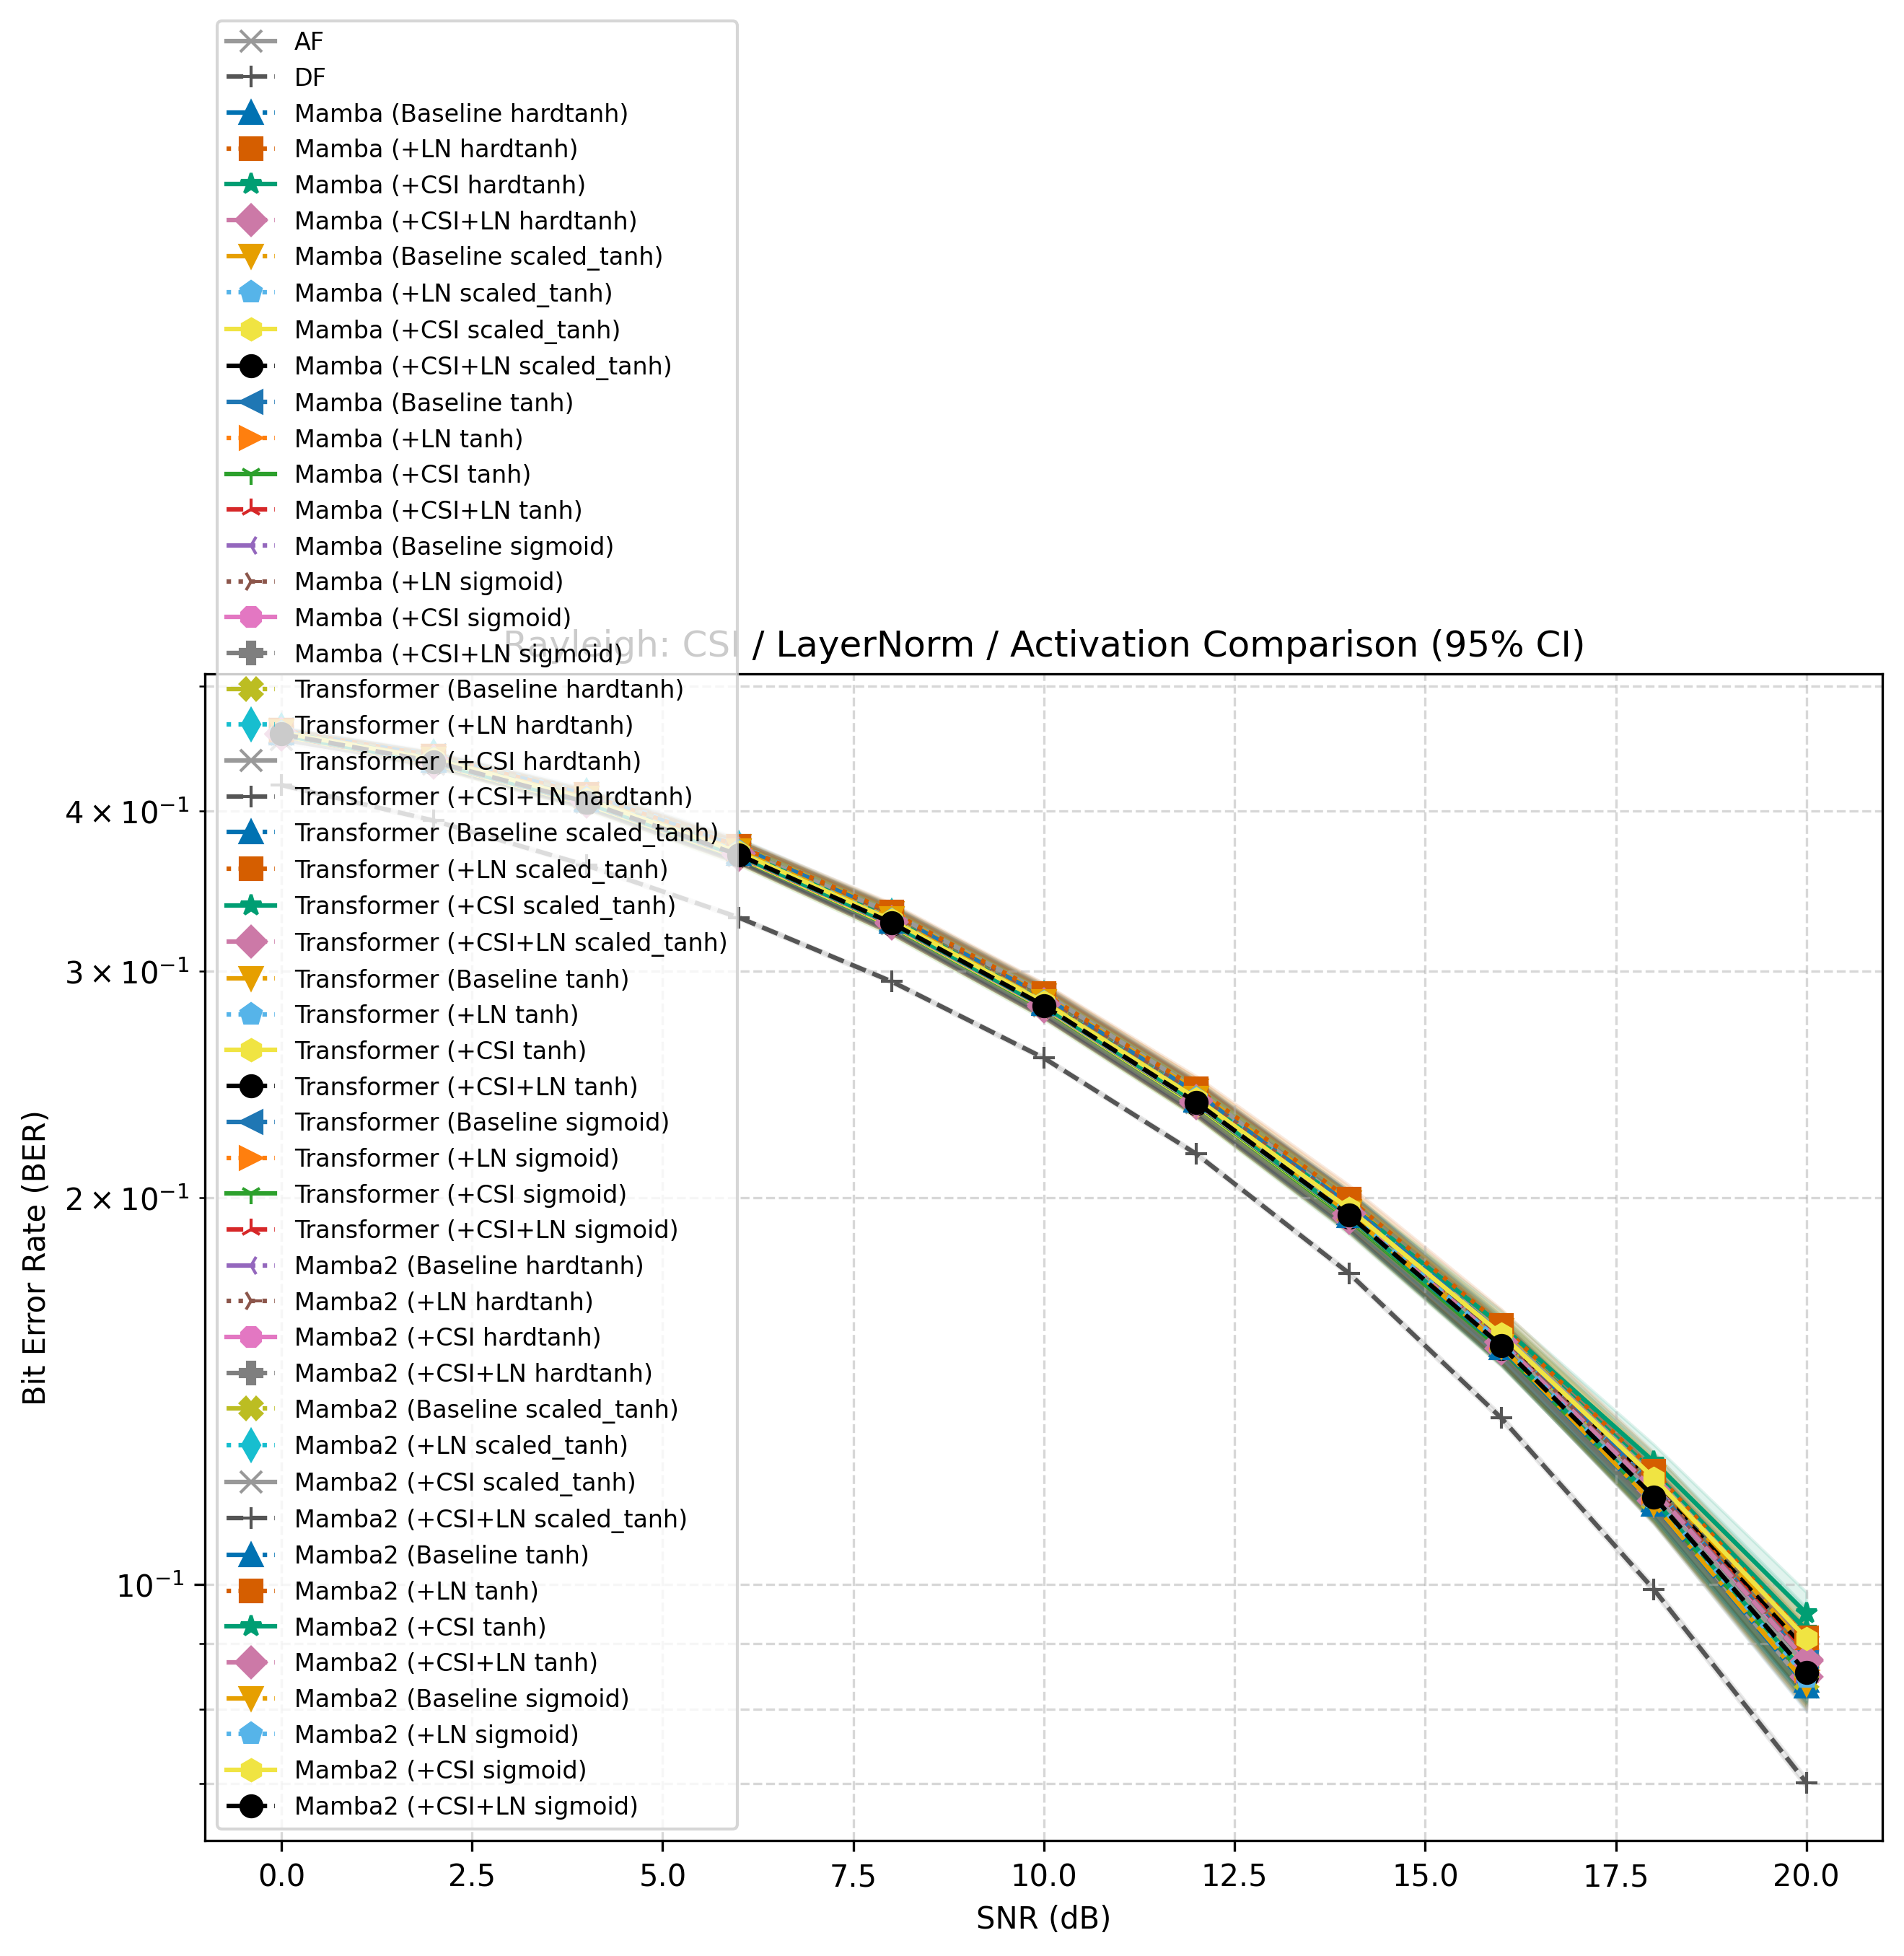
\includegraphics[width=\linewidth,height=0.45\textheight,keepaspectratio]{results/csi/csi_experiment_psk16_rayleigh.png}}
\caption{16-PSK Rayleigh fading --- BER vs.\ SNR for all 48 neural relay variants.}
\label{fig:fig41}
\end{figure}

\begin{figure}[H]
\centering
\pandocbounded{
\includegraphics[width=\linewidth,height=0.45\textheight,keepaspectratio]{results/csi/top3_psk16_rayleigh.png}}
\caption{Top-3 neural relay architectures for 16-PSK in Rayleigh fading. In contrast
to QAM16, all three best-performing PSK16 variants use CSI injection (+CSI or +CSI+LN).}
\label{fig:fig42}
\end{figure}

\begin{figure}[H]
\centering
\pandocbounded{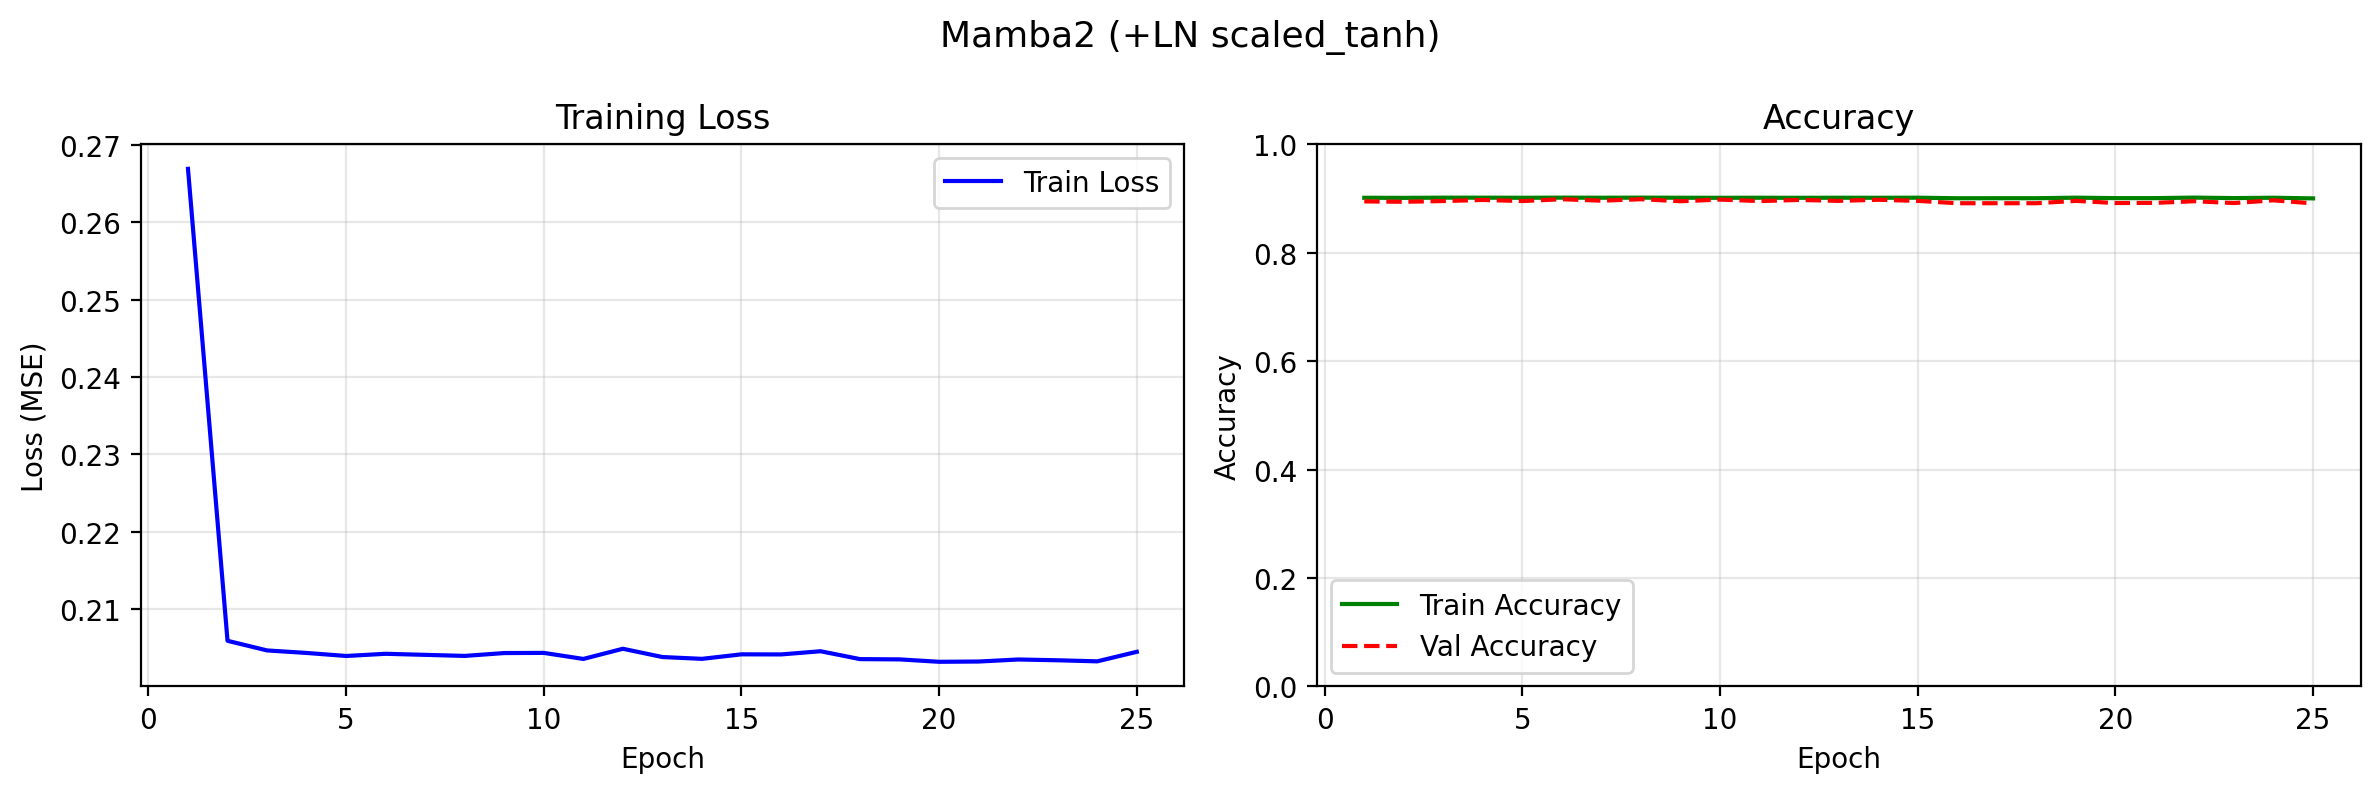
\includegraphics[width=\linewidth,height=0.45\textheight,keepaspectratio]{results/csi/training_Mamba2_LN_scaled_tanh.png}}
\caption{Training loss and accuracy for Mamba-2 (+LN scaled\_tanh). The model converges
within approximately 5 epochs with minimal overfitting.}
\label{fig:fig43}
\end{figure}

\begin{figure}[H]
\centering
\pandocbounded{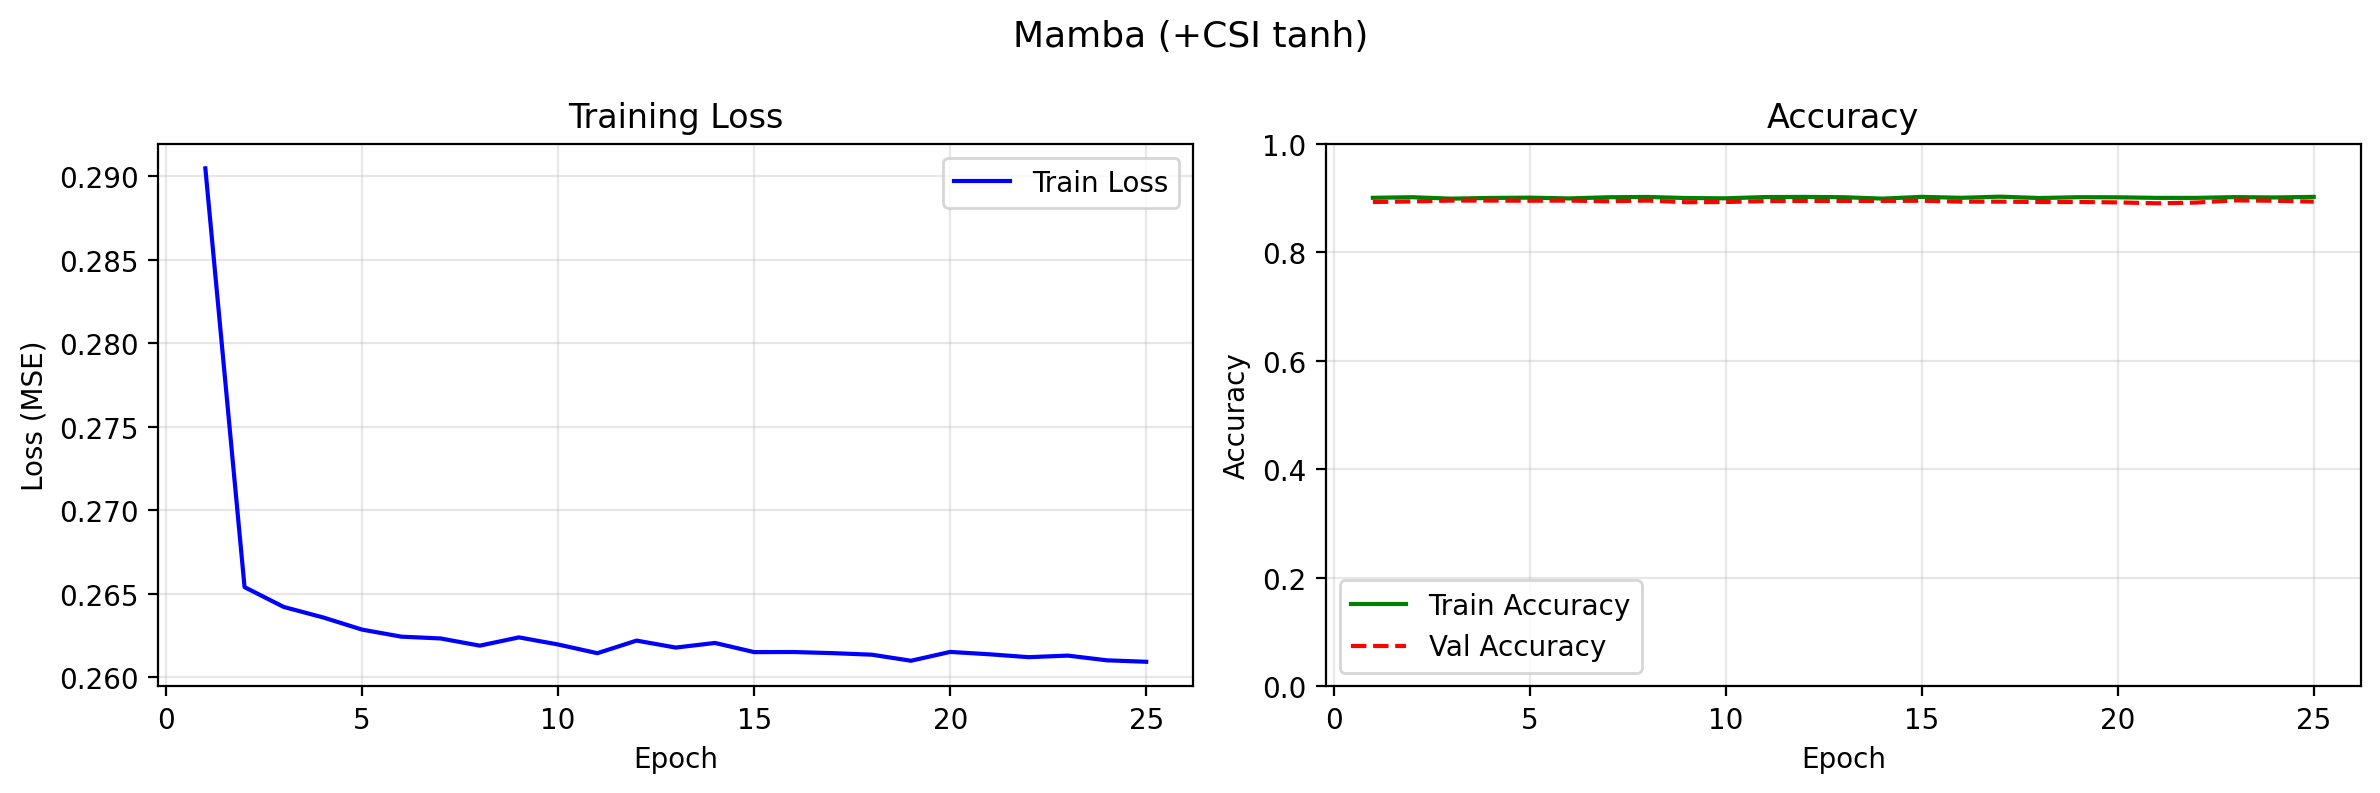
\includegraphics[width=\linewidth,height=0.45\textheight,keepaspectratio]{results/csi/training_Mamba_CSI_tanh.png}}
\caption{Training loss and accuracy for Mamba S6 (+CSI tanh). The CSI-augmented input
produces smooth, monotonic training convergence.}
\label{fig:fig44}
\end{figure}

\begin{figure}[H]
\centering
\pandocbounded{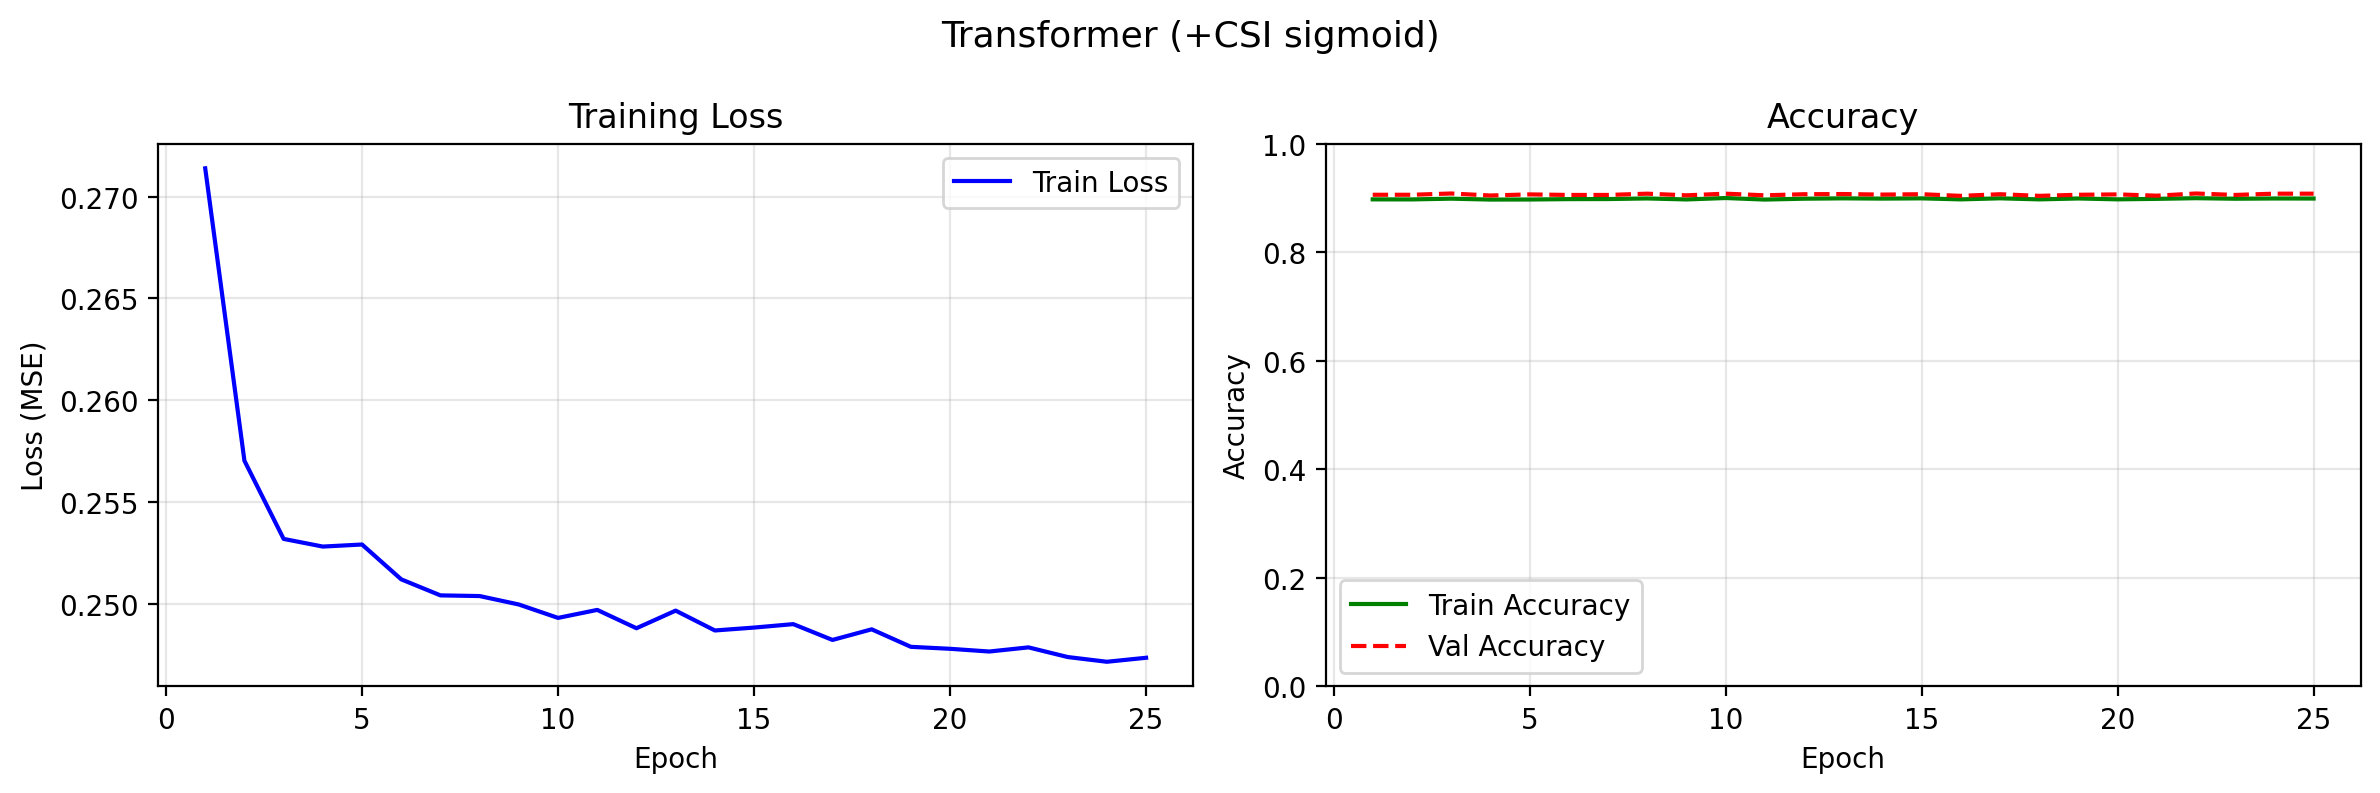
\includegraphics[width=\linewidth,height=0.45\textheight,keepaspectratio]{results/csi/training_Transformer_CSI_sigmoid.png}}
\caption{Training loss and accuracy for Transformer (+CSI sigmoid). Rapid initial
convergence within 3 epochs followed by a flat plateau.}
\label{fig:fig45}
\end{figure}


%% ── E7: 16-Class 2D Classification ──────────────────────────
\section{E7: 16-Class 2D Classification for QAM16}\label{sec:app-e7}

\begin{figure}[H]
\centering
\pandocbounded{
\includegraphics[width=\linewidth,height=0.45\textheight,keepaspectratio]{results/all_relays_16class/ber_all_relays_16class.png}}
\caption{16-QAM BER vs.\ SNR for all relay variants (4-class and 16-class) on AWGN.
The 4-class variants (dashed) plateau at BER $\approx 0.008$ while the 16-class
variants (solid) continue decreasing, approaching and matching the DF baseline.}
\label{fig:fig50}
\end{figure}

\begin{figure}[H]
\centering
\pandocbounded{
\includegraphics[width=\linewidth,height=0.45\textheight,keepaspectratio]{results/all_relays_16class/grouped_bar_16class.png}}
\caption{Grouped bar comparison of 4-class vs.\ 16-class BER at 20\,dB for each
architecture.}
\label{fig:fig51}
\end{figure}

\begin{figure}[H]
\centering
\pandocbounded{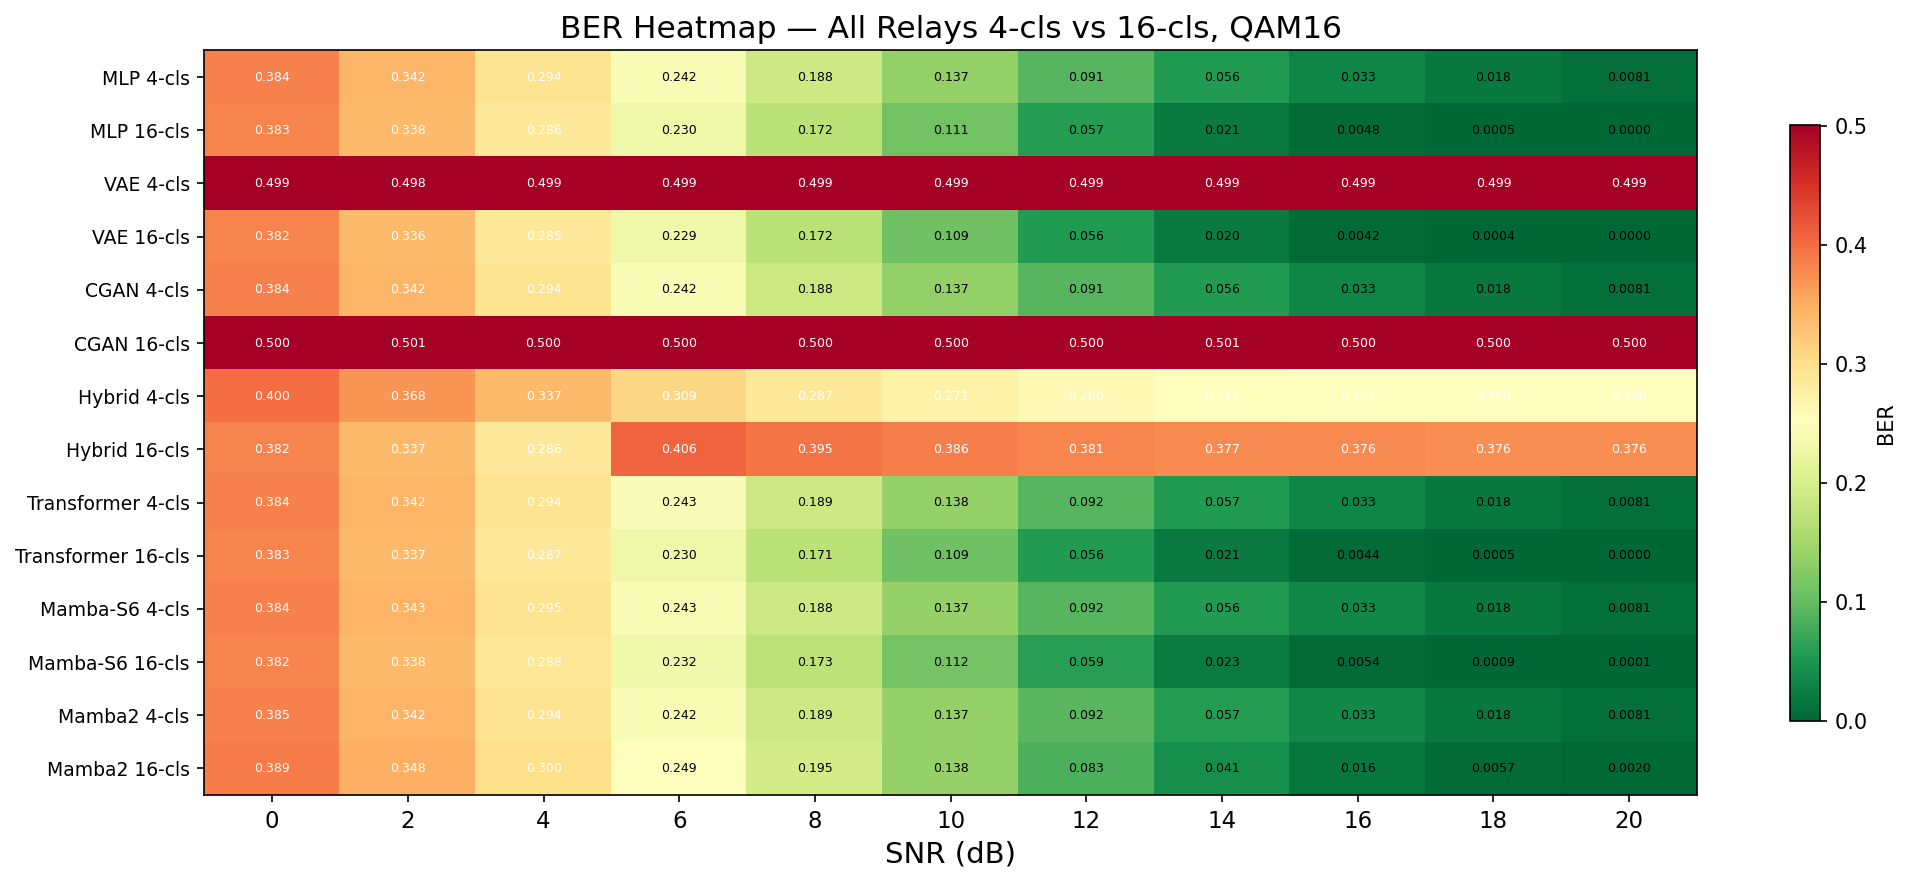
\includegraphics[width=\linewidth,height=0.45\textheight,keepaspectratio]{results/all_relays_16class/heatmap_all_relays_16class.png}}
\caption{Heatmap of BER across all relay variants and SNR points. The 16-class variants
show a clear colour transition from high BER (warm) to near-zero BER (cool) at high SNR.}
\label{fig:fig52}
\end{figure}

\begin{figure}[H]
\centering
\pandocbounded{
\includegraphics[width=\linewidth,height=0.45\textheight,keepaspectratio]{results/all_relays_16class/top3_16class.png}}
\caption{Top-3 16-class relay variants compared against AF and DF. VAE 16-cls,
Transformer 16-cls, and MLP 16-cls all match or approach DF performance.}
\label{fig:fig53}
\end{figure}


%% ── E8: End-to-End Optimisation ─────────────────────────────
\section{E8: End-to-End Joint Optimisation}\label{sec:app-e8}

\begin{figure}[H]
\centering
\pandocbounded{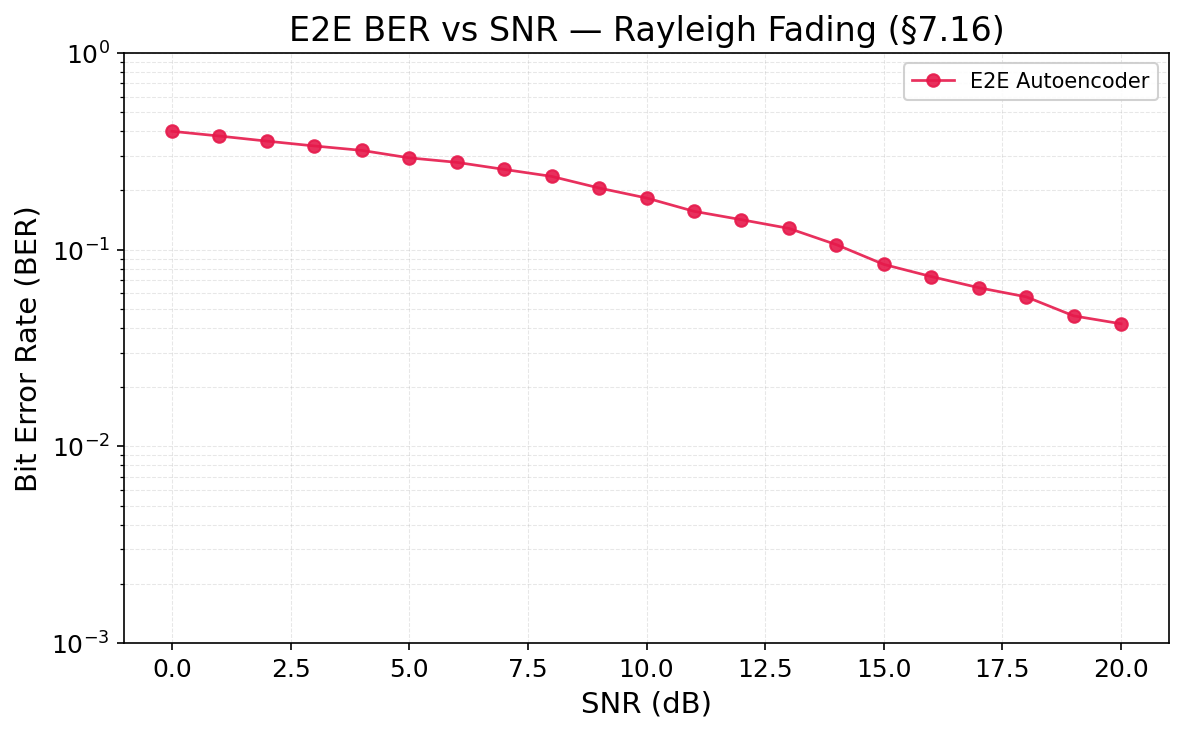
\includegraphics[width=\linewidth,height=0.45\textheight,keepaspectratio]{results/e2e/e2e_ber_comparison.png}}
\caption{BER vs.\ SNR for E2E learned autoencoder compared to theoretical 16-QAM over
Rayleigh fading. The E2E system underperforms the classical grid constellation.}
\label{fig:fig46}
\end{figure}

\begin{figure}[H]
\centering
\pandocbounded{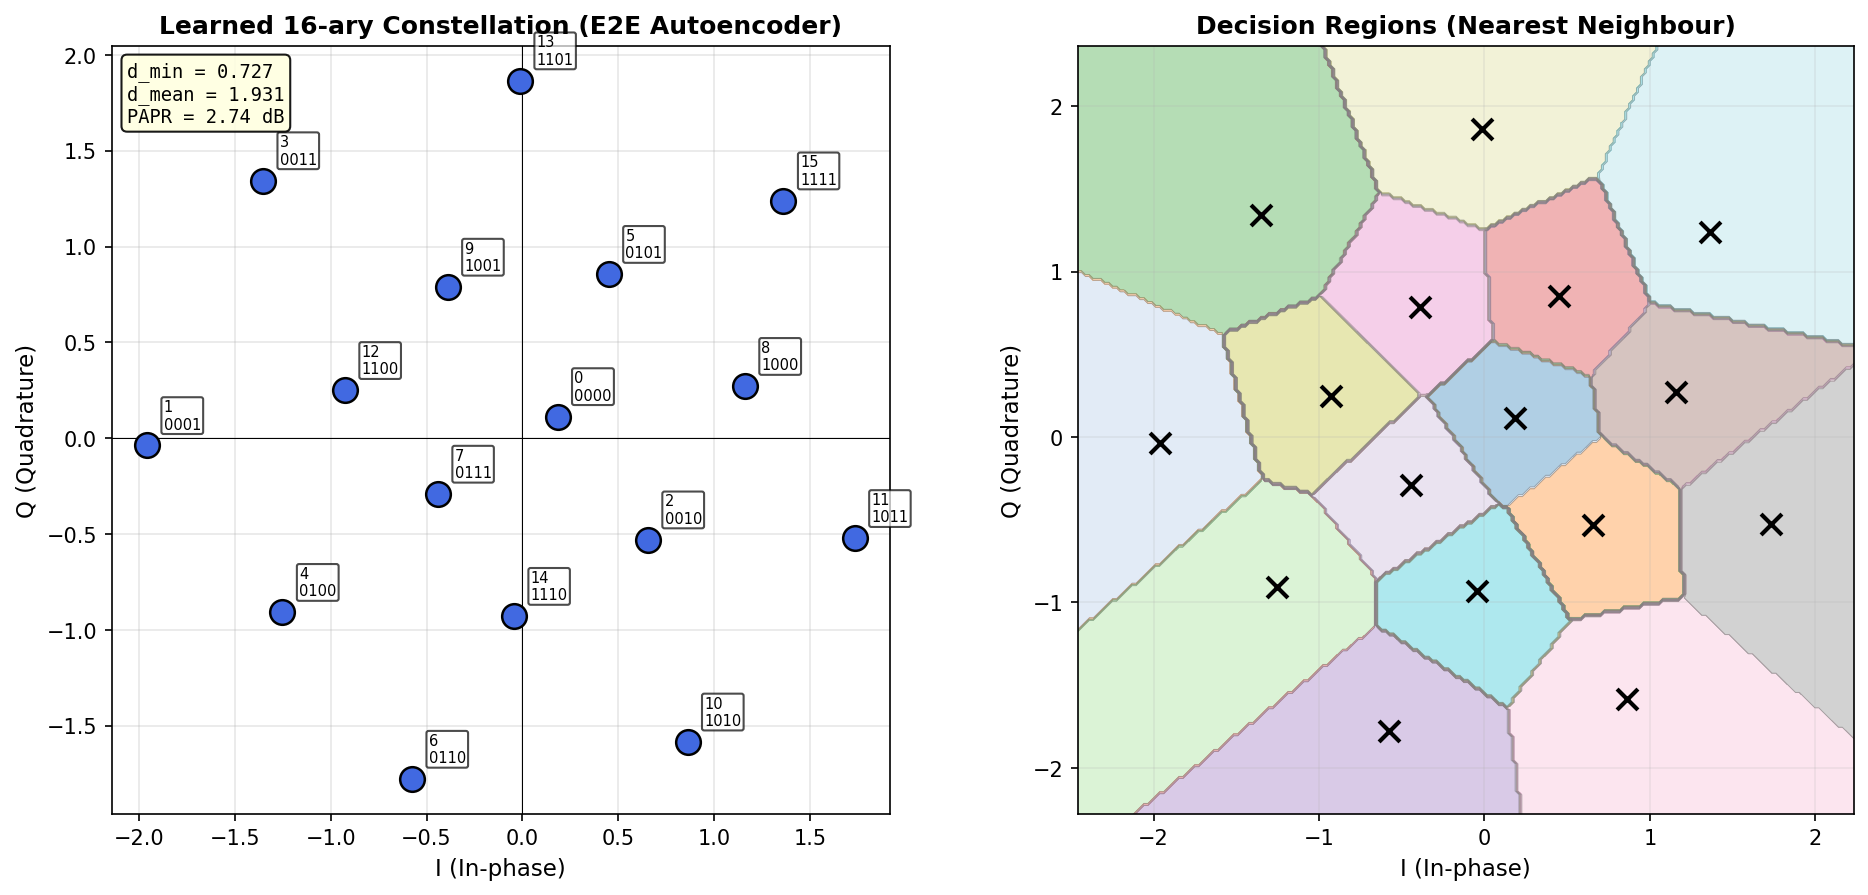
\includegraphics[width=\linewidth,height=0.45\textheight,keepaspectratio]{results/e2e/e2e_constellation.png}}
\caption{Learned 16-point constellation of the E2E autoencoder. The network discovers
a non-rectangular geometry that maximises minimum Euclidean distance.}
\label{fig:fig47}
\end{figure}

\begin{figure}[H]
\centering
\pandocbounded{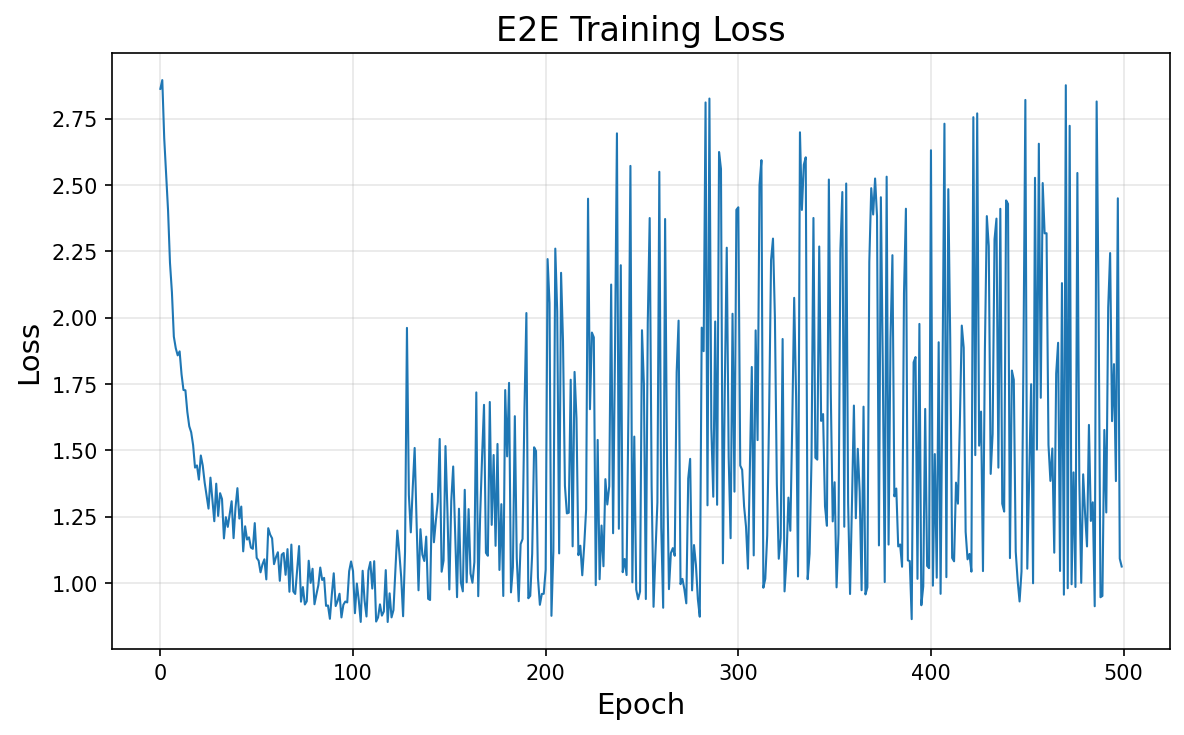
\includegraphics[width=\linewidth,height=0.45\textheight,keepaspectratio]{results/e2e/e2e_training_loss.png}}
\caption{Training loss (cross-entropy) convergence of the E2E autoencoder. The model
converges within approximately 200 epochs.}
\label{fig:fig48}
\end{figure}

\begin{figure}[H]
\centering
\pandocbounded{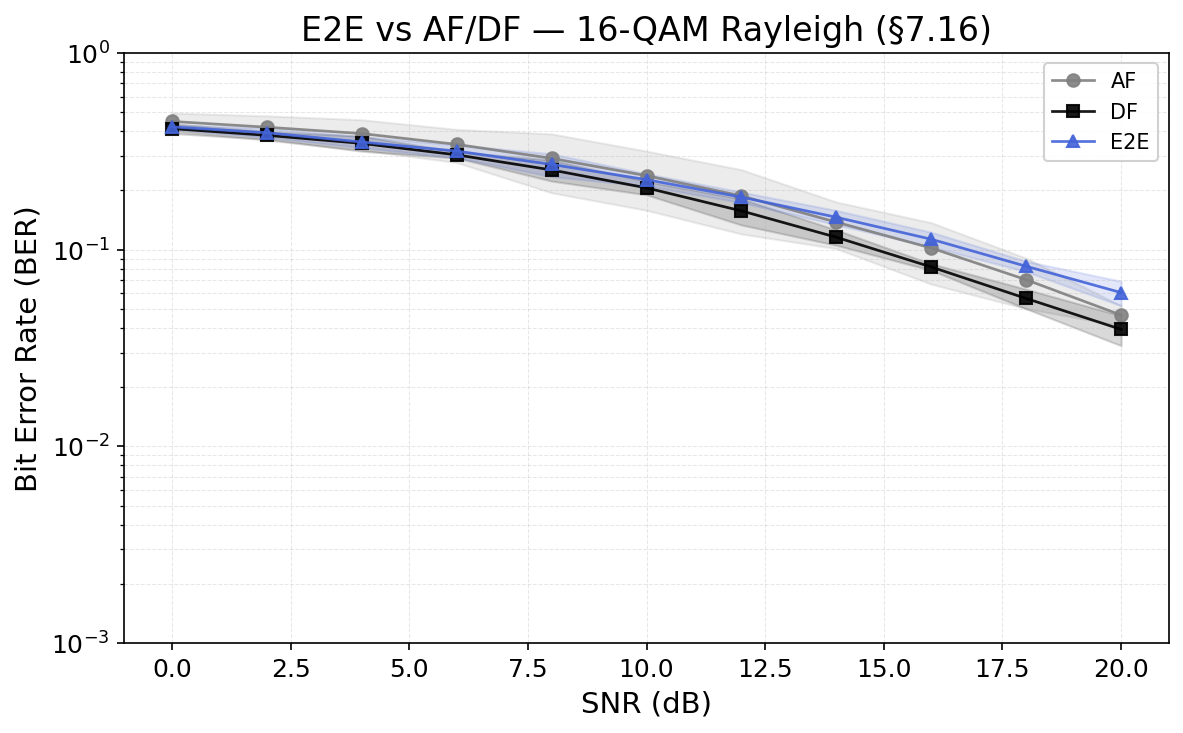
\includegraphics[width=\linewidth,height=0.45\textheight,keepaspectratio]{results/e2e/e2e_relay_comparison.png}}
\caption{Performance comparison of the E2E autoencoder against the modular relay-based
approaches. The E2E system does not achieve lower BER than the two-hop DF relay.}
\label{fig:fig49}
\end{figure}


%% ── Detailed Experimental Tables ────────────────────────────
\section{Detailed Experimental Tables}\label{chap:app-tables}

This section contains the exhaustive numerical BER results for all experiments
described in Chapter~\ref{sec:experiments}.

This appendix contains the exhaustive numerical BER results for the experiments discussed in Chapter~\ref{sec:experiments}.

\begin{longtable}[]{@{}
  >{\raggedright\arraybackslash}p{(\linewidth - 18\tabcolsep) * \real{0.1000}}
  >{\raggedright\arraybackslash}p{(\linewidth - 18\tabcolsep) * \real{0.1000}}
  >{\raggedright\arraybackslash}p{(\linewidth - 18\tabcolsep) * \real{0.1000}}
  >{\raggedright\arraybackslash}p{(\linewidth - 18\tabcolsep) * \real{0.1000}}
  >{\raggedright\arraybackslash}p{(\linewidth - 18\tabcolsep) * \real{0.1000}}
  >{\raggedright\arraybackslash}p{(\linewidth - 18\tabcolsep) * \real{0.1000}}
  >{\raggedright\arraybackslash}p{(\linewidth - 18\tabcolsep) * \real{0.1000}}
  >{\raggedright\arraybackslash}p{(\linewidth - 18\tabcolsep) * \real{0.1000}}
  >{\raggedright\arraybackslash}p{(\linewidth - 18\tabcolsep) * \real{0.1000}}
  >{\raggedright\arraybackslash}p{(\linewidth - 18\tabcolsep) * \real{0.1000}}@{}}
\caption{BER comparison of all nine relay strategies on the AWGN channel.}\label{tbl:table1}\tabularnewline
\toprule\noalign{}
\begin{minipage}[b]{\linewidth}\raggedright
SNR (dB)
\end{minipage} & \begin{minipage}[b]{\linewidth}\raggedright
AF
\end{minipage} & \begin{minipage}[b]{\linewidth}\raggedright
DF
\end{minipage} & \begin{minipage}[b]{\linewidth}\raggedright
MLP (169p)
\end{minipage} & \begin{minipage}[b]{\linewidth}\raggedright
Hybrid
\end{minipage} & \begin{minipage}[b]{\linewidth}\raggedright
VAE
\end{minipage} & \begin{minipage}[b]{\linewidth}\raggedright
CGAN
\end{minipage} & \begin{minipage}[b]{\linewidth}\raggedright
Transformer
\end{minipage} & \begin{minipage}[b]{\linewidth}\raggedright
Mamba S6
\end{minipage} & \begin{minipage}[b]{\linewidth}\raggedright
Mamba-2 SSD
\end{minipage} \\
\midrule\noalign{}
\endfirsthead
\toprule\noalign{}
\begin{minipage}[b]{\linewidth}\raggedright
SNR (dB)
\end{minipage} & \begin{minipage}[b]{\linewidth}\raggedright
AF
\end{minipage} & \begin{minipage}[b]{\linewidth}\raggedright
DF
\end{minipage} & \begin{minipage}[b]{\linewidth}\raggedright
MLP (169p)
\end{minipage} & \begin{minipage}[b]{\linewidth}\raggedright
Hybrid
\end{minipage} & \begin{minipage}[b]{\linewidth}\raggedright
VAE
\end{minipage} & \begin{minipage}[b]{\linewidth}\raggedright
CGAN
\end{minipage} & \begin{minipage}[b]{\linewidth}\raggedright
Transformer
\end{minipage} & \begin{minipage}[b]{\linewidth}\raggedright
Mamba S6
\end{minipage} & \begin{minipage}[b]{\linewidth}\raggedright
Mamba-2 SSD
\end{minipage} \\
\midrule\noalign{}
\endhead
\bottomrule\noalign{}
\endlastfoot
0 & 0.291 & 0.268 & 0.264 & 0.262 & 0.376 & \textbf{0.261} & 0.267 & 0.269 & 0.270 \\
4 & 0.154 & 0.112 & 0.112 & 0.113 & 0.330 & \textbf{0.111} & 0.114 & 0.111 & \textbf{0.111} \\
8 & 0.044 & \textbf{0.010} & 0.015 & \textbf{0.010} & 0.291 & 0.013 & 0.014 & \textbf{0.010} & 0.012 \\
12 & 0.0027 & \textbf{1.67e-04} & \textbf{1.67e-04} & \textbf{1.67e-04} & 0.269 & 3.33e-04 & 3.33e-04 & \textbf{1.67e-04} & \textbf{1.67e-04} \\
16 & \textbf{0} & \textbf{0} & \textbf{0} & \textbf{0} & 0.258 & \textbf{0} & \textbf{0} & \textbf{0} & \textbf{0} \\
20 & \textbf{0} & \textbf{0} & \textbf{0} & \textbf{0} & 0.250 & \textbf{0} & \textbf{0} & \textbf{0} & \textbf{0} \\
\end{longtable}

\begin{longtable}[]{@{}
  >{\raggedright\arraybackslash}p{(\linewidth - 18\tabcolsep) * \real{0.1000}}
  >{\raggedright\arraybackslash}p{(\linewidth - 18\tabcolsep) * \real{0.1000}}
  >{\raggedright\arraybackslash}p{(\linewidth - 18\tabcolsep) * \real{0.1000}}
  >{\raggedright\arraybackslash}p{(\linewidth - 18\tabcolsep) * \real{0.1000}}
  >{\raggedright\arraybackslash}p{(\linewidth - 18\tabcolsep) * \real{0.1000}}
  >{\raggedright\arraybackslash}p{(\linewidth - 18\tabcolsep) * \real{0.1000}}
  >{\raggedright\arraybackslash}p{(\linewidth - 18\tabcolsep) * \real{0.1000}}
  >{\raggedright\arraybackslash}p{(\linewidth - 18\tabcolsep) * \real{0.1000}}
  >{\raggedright\arraybackslash}p{(\linewidth - 18\tabcolsep) * \real{0.1000}}
  >{\raggedright\arraybackslash}p{(\linewidth - 18\tabcolsep) * \real{0.1000}}@{}}
\caption{BER comparison on the Rayleigh fading channel (SISO).}\label{tbl:table2}\tabularnewline
\toprule\noalign{}
\begin{minipage}[b]{\linewidth}\raggedright
SNR (dB)
\end{minipage} & \begin{minipage}[b]{\linewidth}\raggedright
AF
\end{minipage} & \begin{minipage}[b]{\linewidth}\raggedright
DF
\end{minipage} & \begin{minipage}[b]{\linewidth}\raggedright
MLP (169p)
\end{minipage} & \begin{minipage}[b]{\linewidth}\raggedright
Hybrid
\end{minipage} & \begin{minipage}[b]{\linewidth}\raggedright
VAE
\end{minipage} & \begin{minipage}[b]{\linewidth}\raggedright
CGAN
\end{minipage} & \begin{minipage}[b]{\linewidth}\raggedright
Transformer
\end{minipage} & \begin{minipage}[b]{\linewidth}\raggedright
Mamba S6
\end{minipage} & \begin{minipage}[b]{\linewidth}\raggedright
Mamba-2 SSD
\end{minipage} \\
\midrule\noalign{}
\endfirsthead
\toprule\noalign{}
\begin{minipage}[b]{\linewidth}\raggedright
SNR (dB)
\end{minipage} & \begin{minipage}[b]{\linewidth}\raggedright
AF
\end{minipage} & \begin{minipage}[b]{\linewidth}\raggedright
DF
\end{minipage} & \begin{minipage}[b]{\linewidth}\raggedright
MLP (169p)
\end{minipage} & \begin{minipage}[b]{\linewidth}\raggedright
Hybrid
\end{minipage} & \begin{minipage}[b]{\linewidth}\raggedright
VAE
\end{minipage} & \begin{minipage}[b]{\linewidth}\raggedright
CGAN
\end{minipage} & \begin{minipage}[b]{\linewidth}\raggedright
Transformer
\end{minipage} & \begin{minipage}[b]{\linewidth}\raggedright
Mamba S6
\end{minipage} & \begin{minipage}[b]{\linewidth}\raggedright
Mamba-2 SSD
\end{minipage} \\
\midrule\noalign{}
\endhead
\bottomrule\noalign{}
\endlastfoot
0 & 0.330 & \textbf{0.245} & 0.247 & 0.250 & 0.395 & 0.247 & 0.325 & 0.317 & 0.318 \\
4 & 0.205 & 0.139 & 0.141 & 0.141 & 0.347 & \textbf{0.138} & 0.183 & 0.178 & 0.180 \\
8 & 0.092 & \textbf{0.068} & 0.070 & 0.069 & 0.304 & 0.070 & 0.077 & 0.076 & 0.076 \\
12 & 0.037 & \textbf{0.031} & 0.032 & 0.032 & 0.278 & 0.031 & 0.032 & 0.032 & 0.032 \\
16 & 0.015 & 0.014 & 0.014 & 0.014 & 0.262 & 0.014 & 0.014 & \textbf{0.013} & 0.014 \\
20 & 0.0053 & \textbf{0.0047} & \textbf{0.0047} & \textbf{0.0047} & 0.250 & 0.0052 & 0.0048 & 0.0052 & \textbf{0.0047} \\
\end{longtable}

\begin{longtable}[]{@{}
  >{\raggedright\arraybackslash}p{(\linewidth - 18\tabcolsep) * \real{0.1000}}
  >{\raggedright\arraybackslash}p{(\linewidth - 18\tabcolsep) * \real{0.1000}}
  >{\raggedright\arraybackslash}p{(\linewidth - 18\tabcolsep) * \real{0.1000}}
  >{\raggedright\arraybackslash}p{(\linewidth - 18\tabcolsep) * \real{0.1000}}
  >{\raggedright\arraybackslash}p{(\linewidth - 18\tabcolsep) * \real{0.1000}}
  >{\raggedright\arraybackslash}p{(\linewidth - 18\tabcolsep) * \real{0.1000}}
  >{\raggedright\arraybackslash}p{(\linewidth - 18\tabcolsep) * \real{0.1000}}
  >{\raggedright\arraybackslash}p{(\linewidth - 18\tabcolsep) * \real{0.1000}}
  >{\raggedright\arraybackslash}p{(\linewidth - 18\tabcolsep) * \real{0.1000}}
  >{\raggedright\arraybackslash}p{(\linewidth - 18\tabcolsep) * \real{0.1000}}@{}}
\caption{BER comparison on the Rician fading channel with K-factor = 3.}\label{tbl:table3}\tabularnewline
\toprule\noalign{}
\begin{minipage}[b]{\linewidth}\raggedright
SNR (dB)
\end{minipage} & \begin{minipage}[b]{\linewidth}\raggedright
AF
\end{minipage} & \begin{minipage}[b]{\linewidth}\raggedright
DF
\end{minipage} & \begin{minipage}[b]{\linewidth}\raggedright
MLP (169p)
\end{minipage} & \begin{minipage}[b]{\linewidth}\raggedright
Hybrid
\end{minipage} & \begin{minipage}[b]{\linewidth}\raggedright
VAE
\end{minipage} & \begin{minipage}[b]{\linewidth}\raggedright
CGAN
\end{minipage} & \begin{minipage}[b]{\linewidth}\raggedright
Transformer
\end{minipage} & \begin{minipage}[b]{\linewidth}\raggedright
Mamba S6
\end{minipage} & \begin{minipage}[b]{\linewidth}\raggedright
Mamba-2 SSD
\end{minipage} \\
\midrule\noalign{}
\endfirsthead
\toprule\noalign{}
\begin{minipage}[b]{\linewidth}\raggedright
SNR (dB)
\end{minipage} & \begin{minipage}[b]{\linewidth}\raggedright
AF
\end{minipage} & \begin{minipage}[b]{\linewidth}\raggedright
DF
\end{minipage} & \begin{minipage}[b]{\linewidth}\raggedright
MLP (169p)
\end{minipage} & \begin{minipage}[b]{\linewidth}\raggedright
Hybrid
\end{minipage} & \begin{minipage}[b]{\linewidth}\raggedright
VAE
\end{minipage} & \begin{minipage}[b]{\linewidth}\raggedright
CGAN
\end{minipage} & \begin{minipage}[b]{\linewidth}\raggedright
Transformer
\end{minipage} & \begin{minipage}[b]{\linewidth}\raggedright
Mamba S6
\end{minipage} & \begin{minipage}[b]{\linewidth}\raggedright
Mamba-2 SSD
\end{minipage} \\
\midrule\noalign{}
\endhead
\bottomrule\noalign{}
\endlastfoot
0 & 0.265 & 0.206 & 0.206 & 0.205 & 0.372 & \textbf{0.203} & 0.242 & 0.239 & 0.241 \\
4 & 0.137 & \textbf{0.090} & 0.092 & 0.093 & 0.320 & 0.090 & 0.104 & 0.103 & 0.105 \\
8 & 0.044 & \textbf{0.028} & 0.030 & 0.030 & 0.284 & 0.029 & 0.030 & 0.030 & 0.030 \\
12 & 0.0092 & 0.0072 & \textbf{0.0068} & 0.0072 & 0.263 & 0.0077 & 0.0077 & \textbf{0.0068} & 0.0070 \\
16 & 0.0023 & 0.0018 & \textbf{0.0017} & 0.0018 & 0.252 & 0.0018 & 0.0018 & \textbf{0.0017} & \textbf{0.0017} \\
20 & \textbf{6.67e-04} & \textbf{6.67e-04} & \textbf{6.67e-04} & \textbf{6.67e-04} & 0.248 & 8.33e-04 & \textbf{6.67e-04} & \textbf{6.67e-04} & \textbf{6.67e-04} \\
\end{longtable}

\begin{longtable}[]{@{}
  >{\raggedright\arraybackslash}p{(\linewidth - 18\tabcolsep) * \real{0.1000}}
  >{\raggedright\arraybackslash}p{(\linewidth - 18\tabcolsep) * \real{0.1000}}
  >{\raggedright\arraybackslash}p{(\linewidth - 18\tabcolsep) * \real{0.1000}}
  >{\raggedright\arraybackslash}p{(\linewidth - 18\tabcolsep) * \real{0.1000}}
  >{\raggedright\arraybackslash}p{(\linewidth - 18\tabcolsep) * \real{0.1000}}
  >{\raggedright\arraybackslash}p{(\linewidth - 18\tabcolsep) * \real{0.1000}}
  >{\raggedright\arraybackslash}p{(\linewidth - 18\tabcolsep) * \real{0.1000}}
  >{\raggedright\arraybackslash}p{(\linewidth - 18\tabcolsep) * \real{0.1000}}
  >{\raggedright\arraybackslash}p{(\linewidth - 18\tabcolsep) * \real{0.1000}}
  >{\raggedright\arraybackslash}p{(\linewidth - 18\tabcolsep) * \real{0.1000}}@{}}
\caption{BER comparison on 2×2 MIMO Rayleigh channel with ZF equalization.}\label{tbl:table4}\tabularnewline
\toprule\noalign{}
\begin{minipage}[b]{\linewidth}\raggedright
SNR (dB)
\end{minipage} & \begin{minipage}[b]{\linewidth}\raggedright
AF
\end{minipage} & \begin{minipage}[b]{\linewidth}\raggedright
DF
\end{minipage} & \begin{minipage}[b]{\linewidth}\raggedright
MLP (169p)
\end{minipage} & \begin{minipage}[b]{\linewidth}\raggedright
Hybrid
\end{minipage} & \begin{minipage}[b]{\linewidth}\raggedright
VAE
\end{minipage} & \begin{minipage}[b]{\linewidth}\raggedright
CGAN
\end{minipage} & \begin{minipage}[b]{\linewidth}\raggedright
Transformer
\end{minipage} & \begin{minipage}[b]{\linewidth}\raggedright
Mamba S6
\end{minipage} & \begin{minipage}[b]{\linewidth}\raggedright
Mamba-2 SSD
\end{minipage} \\
\midrule\noalign{}
\endfirsthead
\toprule\noalign{}
\begin{minipage}[b]{\linewidth}\raggedright
SNR (dB)
\end{minipage} & \begin{minipage}[b]{\linewidth}\raggedright
AF
\end{minipage} & \begin{minipage}[b]{\linewidth}\raggedright
DF
\end{minipage} & \begin{minipage}[b]{\linewidth}\raggedright
MLP (169p)
\end{minipage} & \begin{minipage}[b]{\linewidth}\raggedright
Hybrid
\end{minipage} & \begin{minipage}[b]{\linewidth}\raggedright
VAE
\end{minipage} & \begin{minipage}[b]{\linewidth}\raggedright
CGAN
\end{minipage} & \begin{minipage}[b]{\linewidth}\raggedright
Transformer
\end{minipage} & \begin{minipage}[b]{\linewidth}\raggedright
Mamba S6
\end{minipage} & \begin{minipage}[b]{\linewidth}\raggedright
Mamba-2 SSD
\end{minipage} \\
\midrule\noalign{}
\endhead
\bottomrule\noalign{}
\endlastfoot
0 & 0.328 & 0.254 & \textbf{0.250} & 0.253 & 0.398 & 0.254 & 0.329 & 0.326 & 0.327 \\
4 & 0.206 & \textbf{0.140} & 0.145 & 0.146 & 0.350 & 0.143 & 0.181 & 0.180 & 0.181 \\
8 & 0.104 & \textbf{0.071} & 0.073 & 0.073 & 0.313 & 0.072 & 0.082 & 0.081 & 0.081 \\
12 & 0.040 & \textbf{0.032} & \textbf{0.032} & \textbf{0.032} & 0.277 & 0.032 & 0.033 & 0.033 & 0.033 \\
16 & 0.015 & 0.014 & \textbf{0.013} & 0.014 & 0.265 & 0.014 & 0.014 & 0.014 & 0.014 \\
20 & 0.0043 & \textbf{0.0037} & 0.0042 & \textbf{0.0037} & 0.256 & \textbf{0.0037} & 0.0038 & 0.0040 & 0.0038 \\
\end{longtable}

\begin{longtable}[]{@{}
  >{\raggedright\arraybackslash}p{(\linewidth - 18\tabcolsep) * \real{0.1000}}
  >{\raggedright\arraybackslash}p{(\linewidth - 18\tabcolsep) * \real{0.1000}}
  >{\raggedright\arraybackslash}p{(\linewidth - 18\tabcolsep) * \real{0.1000}}
  >{\raggedright\arraybackslash}p{(\linewidth - 18\tabcolsep) * \real{0.1000}}
  >{\raggedright\arraybackslash}p{(\linewidth - 18\tabcolsep) * \real{0.1000}}
  >{\raggedright\arraybackslash}p{(\linewidth - 18\tabcolsep) * \real{0.1000}}
  >{\raggedright\arraybackslash}p{(\linewidth - 18\tabcolsep) * \real{0.1000}}
  >{\raggedright\arraybackslash}p{(\linewidth - 18\tabcolsep) * \real{0.1000}}
  >{\raggedright\arraybackslash}p{(\linewidth - 18\tabcolsep) * \real{0.1000}}
  >{\raggedright\arraybackslash}p{(\linewidth - 18\tabcolsep) * \real{0.1000}}@{}}
\caption{BER comparison on 2×2 MIMO Rayleigh channel with MMSE equalization.}\label{tbl:table5}\tabularnewline
\toprule\noalign{}
\begin{minipage}[b]{\linewidth}\raggedright
SNR (dB)
\end{minipage} & \begin{minipage}[b]{\linewidth}\raggedright
AF
\end{minipage} & \begin{minipage}[b]{\linewidth}\raggedright
DF
\end{minipage} & \begin{minipage}[b]{\linewidth}\raggedright
MLP (169p)
\end{minipage} & \begin{minipage}[b]{\linewidth}\raggedright
Hybrid
\end{minipage} & \begin{minipage}[b]{\linewidth}\raggedright
VAE
\end{minipage} & \begin{minipage}[b]{\linewidth}\raggedright
CGAN
\end{minipage} & \begin{minipage}[b]{\linewidth}\raggedright
Transformer
\end{minipage} & \begin{minipage}[b]{\linewidth}\raggedright
Mamba S6
\end{minipage} & \begin{minipage}[b]{\linewidth}\raggedright
Mamba-2 SSD
\end{minipage} \\
\midrule\noalign{}
\endfirsthead
\toprule\noalign{}
\begin{minipage}[b]{\linewidth}\raggedright
SNR (dB)
\end{minipage} & \begin{minipage}[b]{\linewidth}\raggedright
AF
\end{minipage} & \begin{minipage}[b]{\linewidth}\raggedright
DF
\end{minipage} & \begin{minipage}[b]{\linewidth}\raggedright
MLP (169p)
\end{minipage} & \begin{minipage}[b]{\linewidth}\raggedright
Hybrid
\end{minipage} & \begin{minipage}[b]{\linewidth}\raggedright
VAE
\end{minipage} & \begin{minipage}[b]{\linewidth}\raggedright
CGAN
\end{minipage} & \begin{minipage}[b]{\linewidth}\raggedright
Transformer
\end{minipage} & \begin{minipage}[b]{\linewidth}\raggedright
Mamba S6
\end{minipage} & \begin{minipage}[b]{\linewidth}\raggedright
Mamba-2 SSD
\end{minipage} \\
\midrule\noalign{}
\endhead
\bottomrule\noalign{}
\endlastfoot
0 & 0.199 & 0.164 & 0.166 & 0.164 & 0.354 & 0.165 & 0.173 & \textbf{0.163} & 0.165 \\
4 & 0.119 & \textbf{0.086} & 0.090 & \textbf{0.086} & 0.318 & 0.091 & 0.094 & 0.088 & 0.089 \\
8 & 0.058 & \textbf{0.040} & 0.044 & \textbf{0.040} & 0.288 & 0.044 & 0.045 & 0.042 & 0.043 \\
12 & 0.026 & \textbf{0.018} & 0.019 & \textbf{0.018} & 0.270 & 0.019 & 0.020 & 0.018 & 0.019 \\
16 & 0.0090 & \textbf{0.0067} & 0.0073 & \textbf{0.0067} & 0.259 & 0.0072 & 0.0073 & 0.0070 & 0.0070 \\
20 & 0.0020 & 0.0018 & 0.0018 & 0.0018 & 0.255 & 0.0025 & 0.0020 & \textbf{0.0015} & 0.0018 \\
\end{longtable}

\begin{longtable}[]{@{}
  >{\raggedright\arraybackslash}p{(\linewidth - 18\tabcolsep) * \real{0.1000}}
  >{\raggedright\arraybackslash}p{(\linewidth - 18\tabcolsep) * \real{0.1000}}
  >{\raggedright\arraybackslash}p{(\linewidth - 18\tabcolsep) * \real{0.1000}}
  >{\raggedright\arraybackslash}p{(\linewidth - 18\tabcolsep) * \real{0.1000}}
  >{\raggedright\arraybackslash}p{(\linewidth - 18\tabcolsep) * \real{0.1000}}
  >{\raggedright\arraybackslash}p{(\linewidth - 18\tabcolsep) * \real{0.1000}}
  >{\raggedright\arraybackslash}p{(\linewidth - 18\tabcolsep) * \real{0.1000}}
  >{\raggedright\arraybackslash}p{(\linewidth - 18\tabcolsep) * \real{0.1000}}
  >{\raggedright\arraybackslash}p{(\linewidth - 18\tabcolsep) * \real{0.1000}}
  >{\raggedright\arraybackslash}p{(\linewidth - 18\tabcolsep) * \real{0.1000}}@{}}
\caption{BER comparison on 2×2 MIMO Rayleigh channel with MMSE-SIC equalization.}\label{tbl:table6}\tabularnewline
\toprule\noalign{}
\begin{minipage}[b]{\linewidth}\raggedright
SNR (dB)
\end{minipage} & \begin{minipage}[b]{\linewidth}\raggedright
AF
\end{minipage} & \begin{minipage}[b]{\linewidth}\raggedright
DF
\end{minipage} & \begin{minipage}[b]{\linewidth}\raggedright
MLP (169p)
\end{minipage} & \begin{minipage}[b]{\linewidth}\raggedright
Hybrid
\end{minipage} & \begin{minipage}[b]{\linewidth}\raggedright
VAE
\end{minipage} & \begin{minipage}[b]{\linewidth}\raggedright
CGAN
\end{minipage} & \begin{minipage}[b]{\linewidth}\raggedright
Transformer
\end{minipage} & \begin{minipage}[b]{\linewidth}\raggedright
Mamba S6
\end{minipage} & \begin{minipage}[b]{\linewidth}\raggedright
Mamba-2 SSD
\end{minipage} \\
\midrule\noalign{}
\endfirsthead
\toprule\noalign{}
\begin{minipage}[b]{\linewidth}\raggedright
SNR (dB)
\end{minipage} & \begin{minipage}[b]{\linewidth}\raggedright
AF
\end{minipage} & \begin{minipage}[b]{\linewidth}\raggedright
DF
\end{minipage} & \begin{minipage}[b]{\linewidth}\raggedright
MLP (169p)
\end{minipage} & \begin{minipage}[b]{\linewidth}\raggedright
Hybrid
\end{minipage} & \begin{minipage}[b]{\linewidth}\raggedright
VAE
\end{minipage} & \begin{minipage}[b]{\linewidth}\raggedright
CGAN
\end{minipage} & \begin{minipage}[b]{\linewidth}\raggedright
Transformer
\end{minipage} & \begin{minipage}[b]{\linewidth}\raggedright
Mamba S6
\end{minipage} & \begin{minipage}[b]{\linewidth}\raggedright
Mamba-2 SSD
\end{minipage} \\
\midrule\noalign{}
\endhead
\bottomrule\noalign{}
\endlastfoot
0 & 0.172 & \textbf{0.134} & 0.139 & 0.138 & 0.347 & 0.136 & 0.146 & 0.143 & 0.143 \\
4 & 0.075 & \textbf{0.045} & 0.048 & \textbf{0.045} & 0.315 & 0.047 & 0.049 & 0.048 & 0.048 \\
8 & 0.020 & \textbf{0.011} & 0.013 & \textbf{0.011} & 0.290 & 0.012 & 0.012 & 0.012 & 0.012 \\
12 & 0.0052 & \textbf{0.0037} & 0.0038 & \textbf{0.0037} & 0.278 & 0.0043 & 0.0042 & 0.0038 & 0.0038 \\
16 & 0.0017 & 0.0013 & 0.0012 & 0.0013 & 0.271 & 0.0012 & \textbf{0.0010} & 0.0015 & 0.0013 \\
20 & 1.67e-04 & \textbf{0} & \textbf{0} & \textbf{0} & 0.266 & \textbf{0} & \textbf{0} & 1.67e-04 & \textbf{0} \\
\end{longtable}

\begin{longtable}[]{@{}
  >{\raggedright\arraybackslash}p{(\linewidth - 16\tabcolsep) * \real{0.1111}}
  >{\raggedright\arraybackslash}p{(\linewidth - 16\tabcolsep) * \real{0.1111}}
  >{\raggedright\arraybackslash}p{(\linewidth - 16\tabcolsep) * \real{0.1111}}
  >{\raggedright\arraybackslash}p{(\linewidth - 16\tabcolsep) * \real{0.1111}}
  >{\raggedright\arraybackslash}p{(\linewidth - 16\tabcolsep) * \real{0.1111}}
  >{\raggedright\arraybackslash}p{(\linewidth - 16\tabcolsep) * \real{0.1111}}
  >{\raggedright\arraybackslash}p{(\linewidth - 16\tabcolsep) * \real{0.1111}}
  >{\raggedright\arraybackslash}p{(\linewidth - 16\tabcolsep) * \real{0.1111}}
  >{\raggedright\arraybackslash}p{(\linewidth - 16\tabcolsep) * \real{0.1111}}@{}}
\caption{Normalized 3K BER results --- AWGN channel.}\label{tbl:table7}\tabularnewline
\toprule\noalign{}
\begin{minipage}[b]{\linewidth}\raggedright
SNR (dB)
\end{minipage} & \begin{minipage}[b]{\linewidth}\raggedright
MLP-3K
\end{minipage} & \begin{minipage}[b]{\linewidth}\raggedright
Hybrid-3K
\end{minipage} & \begin{minipage}[b]{\linewidth}\raggedright
VAE-3K
\end{minipage} & \begin{minipage}[b]{\linewidth}\raggedright
Transformer-3K
\end{minipage} & \begin{minipage}[b]{\linewidth}\raggedright
Mamba-3K
\end{minipage} & \begin{minipage}[b]{\linewidth}\raggedright
Mamba2-3K
\end{minipage} & \begin{minipage}[b]{\linewidth}\raggedright
AF
\end{minipage} & \begin{minipage}[b]{\linewidth}\raggedright
DF
\end{minipage} \\
\midrule\noalign{}
\endfirsthead
\toprule\noalign{}
\begin{minipage}[b]{\linewidth}\raggedright
SNR (dB)
\end{minipage} & \begin{minipage}[b]{\linewidth}\raggedright
MLP-3K
\end{minipage} & \begin{minipage}[b]{\linewidth}\raggedright
Hybrid-3K
\end{minipage} & \begin{minipage}[b]{\linewidth}\raggedright
VAE-3K
\end{minipage} & \begin{minipage}[b]{\linewidth}\raggedright
Transformer-3K
\end{minipage} & \begin{minipage}[b]{\linewidth}\raggedright
Mamba-3K
\end{minipage} & \begin{minipage}[b]{\linewidth}\raggedright
Mamba2-3K
\end{minipage} & \begin{minipage}[b]{\linewidth}\raggedright
AF
\end{minipage} & \begin{minipage}[b]{\linewidth}\raggedright
DF
\end{minipage} \\
\midrule\noalign{}
\endhead
\bottomrule\noalign{}
\endlastfoot
0 & \textbf{0.267} & 0.269 & 0.408 & 0.269 & 0.271 & 0.270 & 0.291 & 0.268 \\
4 & 0.114 & 0.114 & 0.359 & 0.114 & \textbf{0.112} & 0.113 & 0.154 & 0.112 \\
10 & 0.0033 & \textbf{0.0012} & 0.309 & 0.0023 & 0.0017 & 0.0018 & 0.013 & 0.0012 \\
16 & \textbf{0} & \textbf{0} & 0.285 & \textbf{0} & \textbf{0} & \textbf{0} & 0 & 0 \\
20 & \textbf{0} & \textbf{0} & 0.280 & \textbf{0} & \textbf{0} & \textbf{0} & 0 & 0 \\
\end{longtable}

\begin{longtable}[]{@{}
  >{\raggedright\arraybackslash}p{(\linewidth - 16\tabcolsep) * \real{0.1111}}
  >{\raggedright\arraybackslash}p{(\linewidth - 16\tabcolsep) * \real{0.1111}}
  >{\raggedright\arraybackslash}p{(\linewidth - 16\tabcolsep) * \real{0.1111}}
  >{\raggedright\arraybackslash}p{(\linewidth - 16\tabcolsep) * \real{0.1111}}
  >{\raggedright\arraybackslash}p{(\linewidth - 16\tabcolsep) * \real{0.1111}}
  >{\raggedright\arraybackslash}p{(\linewidth - 16\tabcolsep) * \real{0.1111}}
  >{\raggedright\arraybackslash}p{(\linewidth - 16\tabcolsep) * \real{0.1111}}
  >{\raggedright\arraybackslash}p{(\linewidth - 16\tabcolsep) * \real{0.1111}}
  >{\raggedright\arraybackslash}p{(\linewidth - 16\tabcolsep) * \real{0.1111}}@{}}
\caption{Normalized 3K BER results --- Rayleigh fading channel.}\label{tbl:table8}\tabularnewline
\toprule\noalign{}
\begin{minipage}[b]{\linewidth}\raggedright
SNR (dB)
\end{minipage} & \begin{minipage}[b]{\linewidth}\raggedright
MLP-3K
\end{minipage} & \begin{minipage}[b]{\linewidth}\raggedright
Hybrid-3K
\end{minipage} & \begin{minipage}[b]{\linewidth}\raggedright
VAE-3K
\end{minipage} & \begin{minipage}[b]{\linewidth}\raggedright
Transformer-3K
\end{minipage} & \begin{minipage}[b]{\linewidth}\raggedright
Mamba-3K
\end{minipage} & \begin{minipage}[b]{\linewidth}\raggedright
Mamba2-3K
\end{minipage} & \begin{minipage}[b]{\linewidth}\raggedright
AF
\end{minipage} & \begin{minipage}[b]{\linewidth}\raggedright
DF
\end{minipage} \\
\midrule\noalign{}
\endfirsthead
\toprule\noalign{}
\begin{minipage}[b]{\linewidth}\raggedright
SNR (dB)
\end{minipage} & \begin{minipage}[b]{\linewidth}\raggedright
MLP-3K
\end{minipage} & \begin{minipage}[b]{\linewidth}\raggedright
Hybrid-3K
\end{minipage} & \begin{minipage}[b]{\linewidth}\raggedright
VAE-3K
\end{minipage} & \begin{minipage}[b]{\linewidth}\raggedright
Transformer-3K
\end{minipage} & \begin{minipage}[b]{\linewidth}\raggedright
Mamba-3K
\end{minipage} & \begin{minipage}[b]{\linewidth}\raggedright
Mamba2-3K
\end{minipage} & \begin{minipage}[b]{\linewidth}\raggedright
AF
\end{minipage} & \begin{minipage}[b]{\linewidth}\raggedright
DF
\end{minipage} \\
\midrule\noalign{}
\endhead
\bottomrule\noalign{}
\endlastfoot
0 & \textbf{0.252} & 0.258 & 0.411 & 0.329 & 0.320 & 0.320 & 0.330 & 0.245 \\
4 & 0.146 & \textbf{0.145} & 0.375 & 0.181 & 0.180 & 0.179 & 0.205 & 0.139 \\
10 & 0.049 & \textbf{0.047} & 0.315 & 0.050 & 0.049 & 0.049 & 0.058 & 0.044 \\
16 & 0.015 & 0.014 & 0.289 & 0.014 & \textbf{0.014} & 0.014 & 0.015 & 0.014 \\
20 & 0.0050 & \textbf{0.0047} & 0.279 & \textbf{0.0047} & \textbf{0.0047} & \textbf{0.0047} & 0.0053 & 0.0047 \\
\end{longtable}

\begin{longtable}[]{@{}
  >{\raggedright\arraybackslash}p{(\linewidth - 16\tabcolsep) * \real{0.1111}}
  >{\raggedright\arraybackslash}p{(\linewidth - 16\tabcolsep) * \real{0.1111}}
  >{\raggedright\arraybackslash}p{(\linewidth - 16\tabcolsep) * \real{0.1111}}
  >{\raggedright\arraybackslash}p{(\linewidth - 16\tabcolsep) * \real{0.1111}}
  >{\raggedright\arraybackslash}p{(\linewidth - 16\tabcolsep) * \real{0.1111}}
  >{\raggedright\arraybackslash}p{(\linewidth - 16\tabcolsep) * \real{0.1111}}
  >{\raggedright\arraybackslash}p{(\linewidth - 16\tabcolsep) * \real{0.1111}}
  >{\raggedright\arraybackslash}p{(\linewidth - 16\tabcolsep) * \real{0.1111}}
  >{\raggedright\arraybackslash}p{(\linewidth - 16\tabcolsep) * \real{0.1111}}@{}}
\caption{Normalized 3K BER results --- Rician K=3 fading channel.}\label{tbl:table9}\tabularnewline
\toprule\noalign{}
\begin{minipage}[b]{\linewidth}\raggedright
SNR (dB)
\end{minipage} & \begin{minipage}[b]{\linewidth}\raggedright
MLP-3K
\end{minipage} & \begin{minipage}[b]{\linewidth}\raggedright
Hybrid-3K
\end{minipage} & \begin{minipage}[b]{\linewidth}\raggedright
VAE-3K
\end{minipage} & \begin{minipage}[b]{\linewidth}\raggedright
Transformer-3K
\end{minipage} & \begin{minipage}[b]{\linewidth}\raggedright
Mamba-3K
\end{minipage} & \begin{minipage}[b]{\linewidth}\raggedright
Mamba2-3K
\end{minipage} & \begin{minipage}[b]{\linewidth}\raggedright
AF
\end{minipage} & \begin{minipage}[b]{\linewidth}\raggedright
DF
\end{minipage} \\
\midrule\noalign{}
\endfirsthead
\toprule\noalign{}
\begin{minipage}[b]{\linewidth}\raggedright
SNR (dB)
\end{minipage} & \begin{minipage}[b]{\linewidth}\raggedright
MLP-3K
\end{minipage} & \begin{minipage}[b]{\linewidth}\raggedright
Hybrid-3K
\end{minipage} & \begin{minipage}[b]{\linewidth}\raggedright
VAE-3K
\end{minipage} & \begin{minipage}[b]{\linewidth}\raggedright
Transformer-3K
\end{minipage} & \begin{minipage}[b]{\linewidth}\raggedright
Mamba-3K
\end{minipage} & \begin{minipage}[b]{\linewidth}\raggedright
Mamba2-3K
\end{minipage} & \begin{minipage}[b]{\linewidth}\raggedright
AF
\end{minipage} & \begin{minipage}[b]{\linewidth}\raggedright
DF
\end{minipage} \\
\midrule\noalign{}
\endhead
\bottomrule\noalign{}
\endlastfoot
0 & 0.211 & \textbf{0.211} & 0.389 & 0.243 & 0.242 & 0.241 & 0.265 & 0.206 \\
4 & \textbf{0.095} & 0.099 & 0.345 & 0.104 & 0.102 & 0.103 & 0.137 & 0.090 \\
10 & 0.016 & \textbf{0.015} & 0.301 & 0.016 & 0.016 & 0.016 & 0.020 & 0.015 \\
16 & \textbf{0.0015} & 0.0018 & 0.283 & \textbf{0.0015} & 0.0017 & \textbf{0.0015} & 0.0023 & 0.0018 \\
20 & \textbf{6.67e-04} & \textbf{6.67e-04} & 0.275 & \textbf{6.67e-04} & \textbf{6.67e-04} & \textbf{6.67e-04} & 6.67e-04 & 6.67e-04 \\
\end{longtable}

\begin{longtable}[]{@{}
  >{\raggedright\arraybackslash}p{(\linewidth - 16\tabcolsep) * \real{0.1111}}
  >{\raggedright\arraybackslash}p{(\linewidth - 16\tabcolsep) * \real{0.1111}}
  >{\raggedright\arraybackslash}p{(\linewidth - 16\tabcolsep) * \real{0.1111}}
  >{\raggedright\arraybackslash}p{(\linewidth - 16\tabcolsep) * \real{0.1111}}
  >{\raggedright\arraybackslash}p{(\linewidth - 16\tabcolsep) * \real{0.1111}}
  >{\raggedright\arraybackslash}p{(\linewidth - 16\tabcolsep) * \real{0.1111}}
  >{\raggedright\arraybackslash}p{(\linewidth - 16\tabcolsep) * \real{0.1111}}
  >{\raggedright\arraybackslash}p{(\linewidth - 16\tabcolsep) * \real{0.1111}}
  >{\raggedright\arraybackslash}p{(\linewidth - 16\tabcolsep) * \real{0.1111}}@{}}
\caption{Normalized 3K BER results --- 2×2 MIMO ZF.}\label{tbl:table10}\tabularnewline
\toprule\noalign{}
\begin{minipage}[b]{\linewidth}\raggedright
SNR (dB)
\end{minipage} & \begin{minipage}[b]{\linewidth}\raggedright
MLP-3K
\end{minipage} & \begin{minipage}[b]{\linewidth}\raggedright
Hybrid-3K
\end{minipage} & \begin{minipage}[b]{\linewidth}\raggedright
VAE-3K
\end{minipage} & \begin{minipage}[b]{\linewidth}\raggedright
Transformer-3K
\end{minipage} & \begin{minipage}[b]{\linewidth}\raggedright
Mamba-3K
\end{minipage} & \begin{minipage}[b]{\linewidth}\raggedright
Mamba2-3K
\end{minipage} & \begin{minipage}[b]{\linewidth}\raggedright
AF
\end{minipage} & \begin{minipage}[b]{\linewidth}\raggedright
DF
\end{minipage} \\
\midrule\noalign{}
\endfirsthead
\toprule\noalign{}
\begin{minipage}[b]{\linewidth}\raggedright
SNR (dB)
\end{minipage} & \begin{minipage}[b]{\linewidth}\raggedright
MLP-3K
\end{minipage} & \begin{minipage}[b]{\linewidth}\raggedright
Hybrid-3K
\end{minipage} & \begin{minipage}[b]{\linewidth}\raggedright
VAE-3K
\end{minipage} & \begin{minipage}[b]{\linewidth}\raggedright
Transformer-3K
\end{minipage} & \begin{minipage}[b]{\linewidth}\raggedright
Mamba-3K
\end{minipage} & \begin{minipage}[b]{\linewidth}\raggedright
Mamba2-3K
\end{minipage} & \begin{minipage}[b]{\linewidth}\raggedright
AF
\end{minipage} & \begin{minipage}[b]{\linewidth}\raggedright
DF
\end{minipage} \\
\midrule\noalign{}
\endhead
\bottomrule\noalign{}
\endlastfoot
0 & \textbf{0.256} & 0.257 & 0.410 & 0.329 & 0.327 & 0.326 & 0.328 & 0.254 \\
4 & \textbf{0.146} & 0.150 & 0.369 & 0.185 & 0.181 & 0.182 & 0.206 & 0.140 \\
10 & \textbf{0.049} & 0.049 & 0.319 & 0.053 & 0.052 & 0.053 & 0.066 & 0.048 \\
16 & 0.014 & \textbf{0.014} & 0.288 & 0.014 & 0.014 & 0.014 & 0.015 & 0.014 \\
20 & 0.0040 & \textbf{0.0037} & 0.279 & 0.0040 & 0.0040 & 0.0040 & 0.0043 & 0.0037 \\
\end{longtable}

\begin{longtable}[]{@{}
  >{\raggedright\arraybackslash}p{(\linewidth - 16\tabcolsep) * \real{0.1111}}
  >{\raggedright\arraybackslash}p{(\linewidth - 16\tabcolsep) * \real{0.1111}}
  >{\raggedright\arraybackslash}p{(\linewidth - 16\tabcolsep) * \real{0.1111}}
  >{\raggedright\arraybackslash}p{(\linewidth - 16\tabcolsep) * \real{0.1111}}
  >{\raggedright\arraybackslash}p{(\linewidth - 16\tabcolsep) * \real{0.1111}}
  >{\raggedright\arraybackslash}p{(\linewidth - 16\tabcolsep) * \real{0.1111}}
  >{\raggedright\arraybackslash}p{(\linewidth - 16\tabcolsep) * \real{0.1111}}
  >{\raggedright\arraybackslash}p{(\linewidth - 16\tabcolsep) * \real{0.1111}}
  >{\raggedright\arraybackslash}p{(\linewidth - 16\tabcolsep) * \real{0.1111}}@{}}
\caption{Normalized 3K BER results --- 2×2 MIMO MMSE.}\label{tbl:table11}\tabularnewline
\toprule\noalign{}
\begin{minipage}[b]{\linewidth}\raggedright
SNR (dB)
\end{minipage} & \begin{minipage}[b]{\linewidth}\raggedright
MLP-3K
\end{minipage} & \begin{minipage}[b]{\linewidth}\raggedright
Hybrid-3K
\end{minipage} & \begin{minipage}[b]{\linewidth}\raggedright
VAE-3K
\end{minipage} & \begin{minipage}[b]{\linewidth}\raggedright
Transformer-3K
\end{minipage} & \begin{minipage}[b]{\linewidth}\raggedright
Mamba-3K
\end{minipage} & \begin{minipage}[b]{\linewidth}\raggedright
Mamba2-3K
\end{minipage} & \begin{minipage}[b]{\linewidth}\raggedright
AF
\end{minipage} & \begin{minipage}[b]{\linewidth}\raggedright
DF
\end{minipage} \\
\midrule\noalign{}
\endfirsthead
\toprule\noalign{}
\begin{minipage}[b]{\linewidth}\raggedright
SNR (dB)
\end{minipage} & \begin{minipage}[b]{\linewidth}\raggedright
MLP-3K
\end{minipage} & \begin{minipage}[b]{\linewidth}\raggedright
Hybrid-3K
\end{minipage} & \begin{minipage}[b]{\linewidth}\raggedright
VAE-3K
\end{minipage} & \begin{minipage}[b]{\linewidth}\raggedright
Transformer-3K
\end{minipage} & \begin{minipage}[b]{\linewidth}\raggedright
Mamba-3K
\end{minipage} & \begin{minipage}[b]{\linewidth}\raggedright
Mamba2-3K
\end{minipage} & \begin{minipage}[b]{\linewidth}\raggedright
AF
\end{minipage} & \begin{minipage}[b]{\linewidth}\raggedright
DF
\end{minipage} \\
\midrule\noalign{}
\endhead
\bottomrule\noalign{}
\endlastfoot
0 & 0.167 & \textbf{0.164} & 0.384 & 0.169 & 0.165 & 0.164 & 0.199 & 0.164 \\
4 & 0.094 & \textbf{0.086} & 0.348 & 0.091 & 0.089 & 0.089 & 0.119 & 0.086 \\
10 & 0.030 & 0.027 & 0.317 & 0.029 & \textbf{0.026} & 0.027 & 0.040 & 0.027 \\
16 & 0.0083 & 0.0067 & 0.287 & \textbf{0.0067} & 0.0072 & 0.0073 & 0.0090 & 0.0067 \\
20 & 0.0022 & \textbf{0.0018} & 0.280 & \textbf{0.0018} & \textbf{0.0018} & \textbf{0.0018} & 0.0020 & 0.0018 \\
\end{longtable}

\begin{longtable}[]{@{}
  >{\raggedright\arraybackslash}p{(\linewidth - 16\tabcolsep) * \real{0.1111}}
  >{\raggedright\arraybackslash}p{(\linewidth - 16\tabcolsep) * \real{0.1111}}
  >{\raggedright\arraybackslash}p{(\linewidth - 16\tabcolsep) * \real{0.1111}}
  >{\raggedright\arraybackslash}p{(\linewidth - 16\tabcolsep) * \real{0.1111}}
  >{\raggedright\arraybackslash}p{(\linewidth - 16\tabcolsep) * \real{0.1111}}
  >{\raggedright\arraybackslash}p{(\linewidth - 16\tabcolsep) * \real{0.1111}}
  >{\raggedright\arraybackslash}p{(\linewidth - 16\tabcolsep) * \real{0.1111}}
  >{\raggedright\arraybackslash}p{(\linewidth - 16\tabcolsep) * \real{0.1111}}
  >{\raggedright\arraybackslash}p{(\linewidth - 16\tabcolsep) * \real{0.1111}}@{}}
\caption{Normalized 3K BER results --- 2×2 MIMO SIC.}\label{tbl:table12}\tabularnewline
\toprule\noalign{}
\begin{minipage}[b]{\linewidth}\raggedright
SNR (dB)
\end{minipage} & \begin{minipage}[b]{\linewidth}\raggedright
MLP-3K
\end{minipage} & \begin{minipage}[b]{\linewidth}\raggedright
Hybrid-3K
\end{minipage} & \begin{minipage}[b]{\linewidth}\raggedright
VAE-3K
\end{minipage} & \begin{minipage}[b]{\linewidth}\raggedright
Transformer-3K
\end{minipage} & \begin{minipage}[b]{\linewidth}\raggedright
Mamba-3K
\end{minipage} & \begin{minipage}[b]{\linewidth}\raggedright
Mamba2-3K
\end{minipage} & \begin{minipage}[b]{\linewidth}\raggedright
AF
\end{minipage} & \begin{minipage}[b]{\linewidth}\raggedright
DF
\end{minipage} \\
\midrule\noalign{}
\endfirsthead
\toprule\noalign{}
\begin{minipage}[b]{\linewidth}\raggedright
SNR (dB)
\end{minipage} & \begin{minipage}[b]{\linewidth}\raggedright
MLP-3K
\end{minipage} & \begin{minipage}[b]{\linewidth}\raggedright
Hybrid-3K
\end{minipage} & \begin{minipage}[b]{\linewidth}\raggedright
VAE-3K
\end{minipage} & \begin{minipage}[b]{\linewidth}\raggedright
Transformer-3K
\end{minipage} & \begin{minipage}[b]{\linewidth}\raggedright
Mamba-3K
\end{minipage} & \begin{minipage}[b]{\linewidth}\raggedright
Mamba2-3K
\end{minipage} & \begin{minipage}[b]{\linewidth}\raggedright
AF
\end{minipage} & \begin{minipage}[b]{\linewidth}\raggedright
DF
\end{minipage} \\
\midrule\noalign{}
\endhead
\bottomrule\noalign{}
\endlastfoot
0 & 0.140 & \textbf{0.137} & 0.368 & 0.144 & 0.142 & 0.144 & 0.172 & 0.134 \\
4 & 0.048 & \textbf{0.045} & 0.335 & 0.048 & 0.047 & 0.048 & 0.075 & 0.045 \\
10 & 0.0060 & \textbf{0.0057} & 0.309 & 0.0060 & \textbf{0.0057} & 0.0060 & 0.010 & 0.0057 \\
16 & 0.0013 & 0.0013 & 0.298 & \textbf{0.0010} & 0.0013 & 0.0013 & 0.0017 & 0.0013 \\
20 & 1.67e-04 & \textbf{0} & 0.292 & \textbf{0} & \textbf{0} & \textbf{0} & 1.67e-04 & 0 \\
\end{longtable}

\begin{longtable}[]{@{}
  >{\raggedright\arraybackslash}p{(\linewidth - 10\tabcolsep) * \real{0.1667}}
  >{\raggedright\arraybackslash}p{(\linewidth - 10\tabcolsep) * \real{0.1667}}
  >{\raggedright\arraybackslash}p{(\linewidth - 10\tabcolsep) * \real{0.1667}}
  >{\raggedright\arraybackslash}p{(\linewidth - 10\tabcolsep) * \real{0.1667}}
  >{\raggedright\arraybackslash}p{(\linewidth - 10\tabcolsep) * \real{0.1667}}
  >{\raggedright\arraybackslash}p{(\linewidth - 10\tabcolsep) * \real{0.1667}}@{}}
\caption{Model complexity and timing comparison (experiment-specific training settings; Monte Carlo evaluation over 11 SNR points × 10 trials × 10,000 bits). All inference uses batched window extraction and a single forward pass per signal block.}\label{tbl:table13}\tabularnewline
\toprule\noalign{}
\begin{minipage}[b]{\linewidth}\raggedright
Model
\end{minipage} & \begin{minipage}[b]{\linewidth}\raggedright
Parameters
\end{minipage} & \begin{minipage}[b]{\linewidth}\raggedright
Device
\end{minipage} & \begin{minipage}[b]{\linewidth}\raggedright
Training Time
\end{minipage} & \begin{minipage}[b]{\linewidth}\raggedright
Eval Time (AWGN)
\end{minipage} & \begin{minipage}[b]{\linewidth}\raggedright
Eval Time (SIC)
\end{minipage} \\
\midrule\noalign{}
\endfirsthead
\toprule\noalign{}
\begin{minipage}[b]{\linewidth}\raggedright
Model
\end{minipage} & \begin{minipage}[b]{\linewidth}\raggedright
Parameters
\end{minipage} & \begin{minipage}[b]{\linewidth}\raggedright
Device
\end{minipage} & \begin{minipage}[b]{\linewidth}\raggedright
Training Time
\end{minipage} & \begin{minipage}[b]{\linewidth}\raggedright
Eval Time (AWGN)
\end{minipage} & \begin{minipage}[b]{\linewidth}\raggedright
Eval Time (SIC)
\end{minipage} \\
\midrule\noalign{}
\endhead
\bottomrule\noalign{}
\endlastfoot
AF & 0 & --- & 0 s & 0.80 s & 3.47 s \\
DF & 0 & --- & 0 s & 0.77 s & 1.51 s \\
MLP (169p) & 169 & CPU & 4.9 s & 1.57 s & 2.20 s \\
Hybrid & 169 & CPU & 4.6 s & 0.41 s & 1.70 s \\
VAE & 1,777 & CPU & 21.6 s & 1.81 s & 3.11 s \\
CGAN (WGAN-GP) & 2,946 & CUDA & 7,293 s (\textasciitilde2 h) & 1.14 s & 2.34 s \\
Transformer & 17,697 & CUDA & 474 s (\textasciitilde8 min) & 3.71 s & 3.69 s \\
\textbf{Mamba S6} & \textbf{24,001} & \textbf{CUDA} & \textbf{2,141 s (\textasciitilde36 min)} & \textbf{1.88 s} & \textbf{3.02 s} \\
\textbf{Mamba2 (SSD)} & \textbf{26,179} & \textbf{CUDA} & \textbf{1,438 s (\textasciitilde24 min)} & \textbf{4.11 s} & \textbf{5.61 s} \\
\end{longtable}

\begin{longtable}[]{@{}
  >{\raggedright\arraybackslash}p{(\linewidth - 14\tabcolsep) * \real{0.1250}}
  >{\raggedright\arraybackslash}p{(\linewidth - 14\tabcolsep) * \real{0.1250}}
  >{\raggedright\arraybackslash}p{(\linewidth - 14\tabcolsep) * \real{0.1250}}
  >{\raggedright\arraybackslash}p{(\linewidth - 14\tabcolsep) * \real{0.1250}}
  >{\raggedright\arraybackslash}p{(\linewidth - 14\tabcolsep) * \real{0.1250}}
  >{\raggedright\arraybackslash}p{(\linewidth - 14\tabcolsep) * \real{0.1250}}
  >{\raggedright\arraybackslash}p{(\linewidth - 14\tabcolsep) * \real{0.1250}}
  >{\raggedright\arraybackslash}p{(\linewidth - 14\tabcolsep) * \real{0.1250}}@{}}
\caption{BER comparison across modulations at selected SNR points (AWGN channel). All nine relay strategies.}\label{tbl:table14}\tabularnewline
\toprule\noalign{}
\begin{minipage}[b]{\linewidth}\raggedright
Relay
\end{minipage} & \begin{minipage}[b]{\linewidth}\raggedright
BPSK 0 dB
\end{minipage} & \begin{minipage}[b]{\linewidth}\raggedright
BPSK 10 dB
\end{minipage} & \begin{minipage}[b]{\linewidth}\raggedright
QPSK 0 dB
\end{minipage} & \begin{minipage}[b]{\linewidth}\raggedright
QPSK 10 dB
\end{minipage} & \begin{minipage}[b]{\linewidth}\raggedright
16-QAM 0 dB
\end{minipage} & \begin{minipage}[b]{\linewidth}\raggedright
16-QAM 10 dB
\end{minipage} & \begin{minipage}[b]{\linewidth}\raggedright
16-QAM 16 dB
\end{minipage} \\
\midrule\noalign{}
\endfirsthead
\toprule\noalign{}
\begin{minipage}[b]{\linewidth}\raggedright
Relay
\end{minipage} & \begin{minipage}[b]{\linewidth}\raggedright
BPSK 0 dB
\end{minipage} & \begin{minipage}[b]{\linewidth}\raggedright
BPSK 10 dB
\end{minipage} & \begin{minipage}[b]{\linewidth}\raggedright
QPSK 0 dB
\end{minipage} & \begin{minipage}[b]{\linewidth}\raggedright
QPSK 10 dB
\end{minipage} & \begin{minipage}[b]{\linewidth}\raggedright
16-QAM 0 dB
\end{minipage} & \begin{minipage}[b]{\linewidth}\raggedright
16-QAM 10 dB
\end{minipage} & \begin{minipage}[b]{\linewidth}\raggedright
16-QAM 16 dB
\end{minipage} \\
\midrule\noalign{}
\endhead
\bottomrule\noalign{}
\endlastfoot
AF & 0.2813 & 0.0141 & 0.2794 & 0.0142 & 0.3778 & 0.1244 & 0.0180 \\
DF & 0.2651 & 0.0015 & 0.2644 & 0.0016 & 0.3811 & 0.1076 & 0.0038 \\
MLP (169p) & 0.2589 & 0.0021 & 0.2563 & 0.0025 & 0.3907 & 0.2180 & 0.2180 \\
Hybrid & 0.2573 & 0.0015 & 0.2644 & 0.0016 & 0.4000 & 0.2711 & 0.2512 \\
VAE & 0.2611 & 0.0021 & 0.2597 & 0.0036 & 0.3945 & 0.2391 & 0.2231 \\
CGAN (WGAN-GP) & 0.2633 & 0.0017 & 0.2621 & 0.0018 & 0.3976 & 0.2588 & 0.2486 \\
Transformer & 0.2593 & 0.0024 & 0.2576 & 0.0036 & 0.3897 & 0.2042 & 0.1827 \\
Mamba S6 & 0.2585 & 0.0021 & 0.2560 & 0.0028 & 0.3894 & 0.2016 & 0.1935 \\
Mamba2 (SSD) & 0.2593 & 0.0023 & 0.2566 & 0.0034 & 0.3903 & 0.2032 & 0.1890 \\
\end{longtable}

\begin{longtable}[]{@{}
  >{\raggedright\arraybackslash}p{(\linewidth - 12\tabcolsep) * \real{0.1429}}
  >{\raggedright\arraybackslash}p{(\linewidth - 12\tabcolsep) * \real{0.1429}}
  >{\raggedright\arraybackslash}p{(\linewidth - 12\tabcolsep) * \real{0.1429}}
  >{\raggedright\arraybackslash}p{(\linewidth - 12\tabcolsep) * \real{0.1429}}
  >{\raggedright\arraybackslash}p{(\linewidth - 12\tabcolsep) * \real{0.1429}}
  >{\raggedright\arraybackslash}p{(\linewidth - 12\tabcolsep) * \real{0.1429}}
  >{\raggedright\arraybackslash}p{(\linewidth - 12\tabcolsep) * \real{0.1429}}@{}}
\caption{BER at 16 dB for all relay variants across activation functions and modulations (AWGN and Rayleigh).}\label{tbl:table15}\tabularnewline
\toprule\noalign{}
\begin{minipage}[b]{\linewidth}\raggedright
Relay
\end{minipage} & \begin{minipage}[b]{\linewidth}\raggedright
tanh (BPSK)
\end{minipage} & \begin{minipage}[b]{\linewidth}\raggedright
linear (QAM16)
\end{minipage} & \begin{minipage}[b]{\linewidth}\raggedright
hardtanh (QAM16)
\end{minipage} & \begin{minipage}[b]{\linewidth}\raggedright
tanh (BPSK)
\end{minipage} & \begin{minipage}[b]{\linewidth}\raggedright
linear (QAM16)
\end{minipage} & \begin{minipage}[b]{\linewidth}\raggedright
hardtanh (QAM16)
\end{minipage} \\
\midrule\noalign{}
\endfirsthead
\toprule\noalign{}
\begin{minipage}[b]{\linewidth}\raggedright
Relay
\end{minipage} & \begin{minipage}[b]{\linewidth}\raggedright
tanh (BPSK)
\end{minipage} & \begin{minipage}[b]{\linewidth}\raggedright
linear (QAM16)
\end{minipage} & \begin{minipage}[b]{\linewidth}\raggedright
hardtanh (QAM16)
\end{minipage} & \begin{minipage}[b]{\linewidth}\raggedright
tanh (BPSK)
\end{minipage} & \begin{minipage}[b]{\linewidth}\raggedright
linear (QAM16)
\end{minipage} & \begin{minipage}[b]{\linewidth}\raggedright
hardtanh (QAM16)
\end{minipage} \\
\midrule\noalign{}
\endhead
\bottomrule\noalign{}
\endlastfoot
& \textbf{AWGN} & & & \textbf{Rayleigh} & & \\
MLP & 0.2202 & 0.0721 & \textbf{0.0630} & 0.2375 & 0.1279 & \textbf{0.1247} \\
Hybrid & 0.2512 & 0.2512 & 0.2512 & 0.2723 & 0.2723 & 0.2723 \\
VAE & 0.2231 & 0.1111 & \textbf{0.1059} & 0.2462 & 0.1575 & \textbf{0.1573} \\
CGAN & 0.2482 & 0.0973 & \textbf{0.0863} & 0.2666 & 0.1432 & \textbf{0.1383} \\
Transformer & 0.2111 & \textbf{0.0453} & 0.0505 & 0.2305 & \textbf{0.1159} & 0.1194 \\
Mamba S6 & 0.2131 & 0.0422 & \textbf{0.0396} & 0.2333 & 0.1129 & \textbf{0.1108} \\
Mamba-2 SSD & 0.2065 & 0.0471 & \textbf{0.0441} & 0.2273 & 0.1157 & \textbf{0.1145} \\
AF & 0.0180 & --- & --- & 0.1009 & --- & --- \\
DF & 0.0038 & --- & --- & 0.0828 & --- & --- \\
\end{longtable}

\begin{longtable}[]{@{}
  >{\raggedright\arraybackslash}p{(\linewidth - 8\tabcolsep) * \real{0.2000}}
  >{\raggedright\arraybackslash}p{(\linewidth - 8\tabcolsep) * \real{0.2000}}
  >{\raggedright\arraybackslash}p{(\linewidth - 8\tabcolsep) * \real{0.2000}}
  >{\raggedright\arraybackslash}p{(\linewidth - 8\tabcolsep) * \real{0.2000}}
  >{\raggedright\arraybackslash}p{(\linewidth - 8\tabcolsep) * \real{0.2000}}@{}}
\caption{16-QAM BER improvements at 20 dB for sequence models with and without CSI injection and layer normalisation (AWGN).}\label{tbl:table16}\tabularnewline
\toprule\noalign{}
\begin{minipage}[b]{\linewidth}\raggedright
SNR (dB)
\end{minipage} & \begin{minipage}[b]{\linewidth}\raggedright
AF Baseline
\end{minipage} & \begin{minipage}[b]{\linewidth}\raggedright
DF Baseline
\end{minipage} & \begin{minipage}[b]{\linewidth}\raggedright
Mamba S6 (Baseline)
\end{minipage} & \begin{minipage}[b]{\linewidth}\raggedright
Mamba S6 (+CSI + LN)
\end{minipage} \\
\midrule\noalign{}
\endfirsthead
\toprule\noalign{}
\begin{minipage}[b]{\linewidth}\raggedright
SNR (dB)
\end{minipage} & \begin{minipage}[b]{\linewidth}\raggedright
AF Baseline
\end{minipage} & \begin{minipage}[b]{\linewidth}\raggedright
DF Baseline
\end{minipage} & \begin{minipage}[b]{\linewidth}\raggedright
Mamba S6 (Baseline)
\end{minipage} & \begin{minipage}[b]{\linewidth}\raggedright
Mamba S6 (+CSI + LN)
\end{minipage} \\
\midrule\noalign{}
\endhead
\bottomrule\noalign{}
\endlastfoot
\textbf{0.0} & 0.3332 & 0.4300 & 0.2288 & 0.2396 \\
\textbf{8.0} & 0.1436 & 0.2798 & 0.2241 & 0.0635 \\
\textbf{14.0} & 0.0592 & 0.1557 & 0.2227 & 0.0163 \\
\textbf{20.0} & 0.0246 & 0.0901 & 0.2302 & \textbf{0.0055} \\
\end{longtable}

\begin{longtable}[]{@{}llll@{}}
\caption{BER at 20 dB for all relay variants: 4-class (I/Q split) vs.~16-class (joint 2D) classification for 16-QAM.}\label{tbl:table24}\tabularnewline
\toprule\noalign{}
Relay & 4-cls BER @ 20 dB & 16-cls BER @ 20 dB & Improvement \\
\midrule\noalign{}
\endfirsthead
\toprule\noalign{}
Relay & 4-cls BER @ 20 dB & 16-cls BER @ 20 dB & Improvement \\
\midrule\noalign{}
\endhead
\bottomrule\noalign{}
\endlastfoot
MLP & 0.00811 & \textbf{0.00002} & 405× \\
VAE & --- & \textbf{0.00000} & --- \\
CGAN & 0.00811 & --- & --- \\
Hybrid & --- & --- & --- \\
Transformer & 0.00810 & \textbf{0.00001} & 810× \\
Mamba S6 & 0.00810 & \textbf{0.00009} & 90× \\
Mamba-2 SSD & 0.00811 & \textbf{0.00197} & 4.1× \\
AF & 0.00063 & --- & --- \\
DF & 0.00000 & --- & --- \\
\end{longtable}